\documentclass[a4paper,11pt,twoside]{report}
\graphicspath{{images/}}

\usepackage{amssymb}
\usepackage{amsmath}
\usepackage{polski}
\usepackage[utf8]{inputenc}
\usepackage{hyperref}
\usepackage{blindtext}
\usepackage{multicol}
\usepackage{multirow}
\usepackage{wrapfig}
\usepackage{float}
\usepackage{enumitem}
\usepackage{xfrac}
\usepackage{caption}
\usepackage{subcaption}
\usepackage{booktabs}
\usepackage{wasysym}
\usepackage{xcolor}
\usepackage{pdfpages}
\usepackage{fontspec}
\usepackage{comment}
\usepackage{tocloft}
\usepackage{listings}
\usepackage{times}
\usepackage{amsmath}
\usepackage{bm}
\lstset{basicstyle=\ttfamily, columns=fullflexible}

\usepackage{caption, copyrightbox}
\captionsetup{justification=centering, labelfont=sc, labelsep=endash}

\usepackage{regexpatch}
\usepackage[os=mac]{menukeys}
\renewmenumacro{\keys}[+]{shadowedroundedkeys}
\renewmenumacro{\menu}[>]{angularmenus}
\xpatchcmd*{\SPACE}{2em}{1em}{}{}

\definecolor{quotationcolour}{HTML}{F0F0F0}
\definecolor{quotationmarkcolour}{HTML}{1F3F81}

% Double-line for start and end of epigraph.
\newcommand{\epiline}{\hrule \vskip -.2em \hrule}
% Massively humongous opening quotation mark.
\newcommand{\hugequote}{%
  \fontsize{42}{48}\selectfont \color{quotationmarkcolour} \textbf{``}
  \vskip -.5em
}

% Beautify quotations.
\newcommand{\epigraph}[2]{%
  \bigskip
  \begin{center}
  \colorbox{quotationcolour}{%
    \parbox{.80\textwidth}{%
    \epiline \vskip 1em {\hugequote} \vskip -.5em
    \parindent 2.2em
    #1\vspace{-.25cm}\begin{flushright}\textsc{#2}\end{flushright}
    \epiline
    }
  }
  \end{center}
  \bigskip
}

\setmainfont{Verdana}

\addtolength{\cftsecnumwidth}{5pt}
\addtolength{\cftsubsecnumwidth}{5pt}
\addtolength{\cftsubsubsecnumwidth}{5pt}
	
\usepackage{color, colortbl}
\definecolor{Gray}{gray}{0.9}

\definecolor{mGreen}{rgb}{0,0.6,0}
\definecolor{mGray}{rgb}{0.5,0.5,0.5}
\definecolor{mPurple}{rgb}{0.58,0,0.82}
\definecolor{backgroundColour}{rgb}{0.95,0.95,0.92}

\lstdefinestyle{CStyle}{
    backgroundcolor=\color{backgroundColour},   
    commentstyle=\color{mGreen},
    keywordstyle=\color{magenta},
    numberstyle=\tiny\color{mGray},
    stringstyle=\color{mPurple},
    basicstyle=\footnotesize,
    breakatwhitespace=false,         
    breaklines=true,                 
    captionpos=b,                    
    keepspaces=true,                 
    numbers=left,                    
    numbersep=5pt,                  
    showspaces=false,                
    showstringspaces=false,
    showtabs=false,                  
    tabsize=2,
    language=C
}

\usepackage[
backend=biber
,style=ieee
,sorting=none
]{biblatex}
\addbibresource{bibliografia.bib}
\DeclareNameAlias{author}{last-first}

\DeclareCiteCommand{\supercite}[\mkbibsuperscript]
  {\iffieldundef{prenote}
     {}
     {\BibliographyWarning{Ignoring prenote argument}}%
   \iffieldundef{postnote}
     {}
     {\BibliographyWarning{Ignoring postnote argument}}}
  {\usebibmacro{citeindex}%
   \bibopenbracket\usebibmacro{cite}\bibclosebracket}
  {\supercitedelim}
  {}
  
  \DeclareLabelalphaTemplate{
  \labelelement{
    \field[final]{shorthand}
    \field{label}
    \field[strwidth=3,strside=left,ifnames=1]{labelname}
    \field[strwidth=1,strside=left,final]{labelname}
    \field{labeltitle}
  }
  \labelelement{
    \field[strwidth=2,strside=right]{year}
  }
}

\renewcommand*{\figurename}{Rys.}

\usepackage{titlesec}
\titlelabel{\thetitle.\quad}

\usepackage{tikz}


\usetikzlibrary{matrix, ,backgrounds}
\usepackage{array}

\makeatletter
\tikzset{SWOT/.style={matrix of nodes,inner sep=0pt,row sep=0pt,column sep=0pt,
cells={nodes={anchor=center,inner sep=2pt}},
column 1/.style={nodes={rotate=90,minimum height=8mm}},
ampersand replacement=\&,
execute at end matrix={\begin{scope}[on background layer]
 \fill[black!10] (\tikz@fig@name.west|-\tikz@fig@name-2-2.north) rectangle 
  (\tikz@fig@name-\the\pgfmatrixcurrentrow-2.south west);
\end{scope}
\draw (\tikz@fig@name.west|-\tikz@fig@name-2-2.north) rectangle 
(\tikz@fig@name-\the\pgfmatrixcurrentrow-\the\pgfmatrixcurrentcolumn.south east)
 (\tikz@fig@name-1-2.north west) rectangle 
(\tikz@fig@name-\the\pgfmatrixcurrentrow-\the\pgfmatrixcurrentcolumn.south east)
(\tikz@fig@name-2-2.center|-\tikz@fig@name.north) --
 (\tikz@fig@name-2-2.center|-\tikz@fig@name.south)
foreach \XX in {2,...,\the\numexpr\pgfmatrixcurrentrow-1}
{(\tikz@fig@name-\XX-2.south-|\tikz@fig@name.west) --
(\tikz@fig@name-\XX-2.south-|\tikz@fig@name.east) };
}}}
\makeatother

\usepackage{tocloft}
\renewcommand\cftfigfont{\small}

\setlength{\parindent}{0pt}


% -------------------------- USER SETTINGS ---------------------------

\newcommand{\tytul}{Zastosowanie nawigacji inercjalnej do pomiaru pozycji i orientacji w układach robotycznych}
\renewcommand{\title}{Adaptation of inertial navigation for position and orientation measurements in robotic systems}
\newcommand{\type}{Master} % Master OR Engineer
\newcommand{\supervisor}{Marek Wojtyra, D.Sc., Ph.D., M.Eng.} % TITLE AND NAME OF THE SUPERVISOR

\begin{document}
\sloppy
\selectlanguage{english}

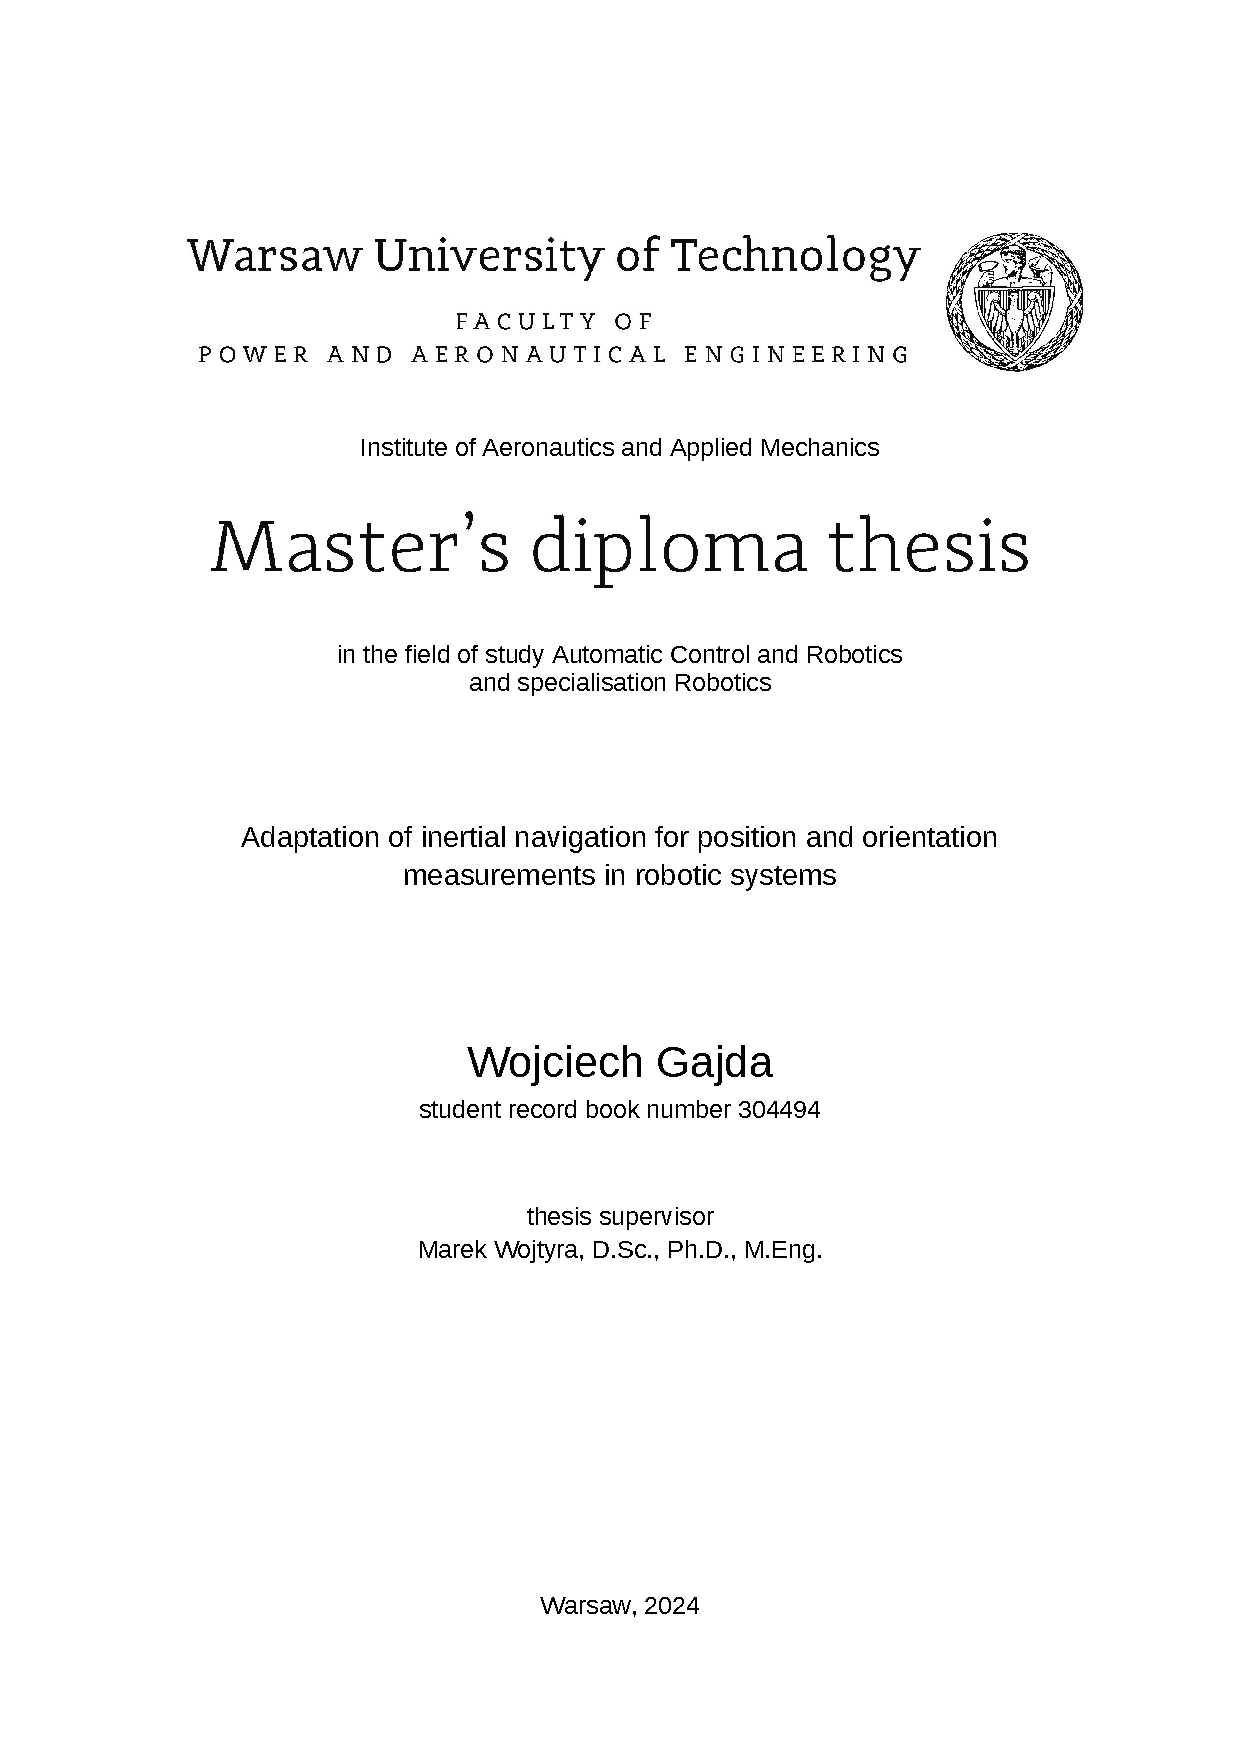
\includepdf[pages=1]{titlepage}
\null\thispagestyle{empty}\newpage

% ---------------------------- ABSTRACTS -----------------------------

{  \fontsize{12}{14} \selectfont
	\begin{abstract}
		
		\begin{center}
			\title
		\end{center}
		
		The thesis describes an implementation of a system designed to estimate the position and orientation of a mechanism, robot, or similar machine based mainly on inertial sensor measurements. The system allows for conducting real-time estimation based on diverse data sources. Moreover, the system takes into account information regarding the mechanical design and the imposed motion constraints. The system operation results in real-time visualization and a set of recorded logs, allowing for subsequent analysis.\\
		
		The work gathered and systematized knowledge about sensors, methods of filtering their measurements, and techniques of measurement fusion. Based on the collected information, a Kalman filter model was developed, allowing efficient estimation of the mechanism parts' position and
		orientation. An important novelty is the proposal of a modification introduced to the method embedded in the Kalman filter, aiming at taking into account the constraints imposed on the state variables. Theoretical considerations found counterparts in the actual implementation, the functioning of which was analyzed using a selected test case.\\
		
		\noindent \textbf{Keywords:} estimation, sensors, filtering, sensor fusion, constraints, Extended Kalman Filter
	\end{abstract}
}

\null\thispagestyle{empty}\newpage


{\selectlanguage{polish} \fontsize{12}{14}\selectfont
	\begin{abstract}
		
		\begin{center}
			\tytul
		\end{center}
		
		W pracy opisano realizację systemu przeznaczonego do estymacji pozycji i~orientacji mechanizmów, robotów i podobnych maszyn, bazującego w głównej mierze na pomiarach czujników inercjalnych. System pozwala na prowadzenie estymacji w~czasie rzeczywistym w~oparciu o~zróżnicowane źródła danych. Ponadto w~systemie uwzględniona została informacja o konstrukcji mechanicznej i~ograniczeniach jej ruchu. Wynikiem działania systemu jest wizualizacja w~czasie rzeczywistym oraz zbiór zarejestrowanych danych, pozwalających na późniejszą analizę.\\
		
		W ramach pracy zgromadzono i~uporządkowano wiedzę na temat czujników pomiarowych, metod filtracji ich pomiarów i~metod fuzji pomiarów.
		Bazując na przygotowanych informacjach opracowano model filtru Kalmana, pozwalający na efektywną estymację pozycji i~orientacji członów mechanizmu. Istotną nowością jest zaproponowanie modyfikacji osadzonej w filtrze Kalmana, umożliwiającej uwzględnienie więzów krępujących zmienne stanu. Rozważania teoretyczne znalazły odzwierciedlenie w rzeczywistej implementacji, której działanie przeanalizowano na wybranym przypadku badawczym.\\
		
		
		\noindent \textbf{Słowa kluczowe:} estymacja, czujniki, filtracja, fuzja czujników, więzy, rozszerzony filtr Kalmana
	\end{abstract}
}

\null\thispagestyle{empty}\newpage

% ------------------- TABLE OF CONTENTS ---------------------
% \selectlanguage{english} - for English
\pagenumbering{gobble}
\tableofcontents
\thispagestyle{empty}
\newpage % IF YOU HAVE EVEN QUANTITY OD PAGES OF TOC, THEN REMOVE IT OR ADD \null\newpage FOR DOUBLE BLANK PAGE BEFORE INTRODUCTION



% -------------------- THE BODY OF THE THESIS --------------------------------

\null\thispagestyle{empty}\newpage
\pagestyle{fancy}
\pagenumbering{arabic}
\setcounter{page}{10}

\chapter{Introduction}

\section{Motivation}

The motivation behind this thesis stems from a research project dedicated to creating hybrid, i.e., exploiting rigid-flexible models, methods for analyzing overconstrained multi-body systems. Research conducted in this project is planned to be validated in an experimental study. The test bench prepared for this purpose is being successively upgraded to meet various requirements. Specifically, the experimental setup needs to be equipped with position and orientation measuring sensors. Fulfilling this demand poses a significant challenge, particularly when attempting to measure forces in dynamic scenarios. Encoders planted in actuators cannot be used since it is planned to make the test bed externally driven by an industrial robotic manipulator). Moreover, installing motion measuring devices in the joints of the mechanism might hamper -- crucial for the project -- joint reaction forces measurements. The need to correlate position and orientation data with force measurements led to considerations of how measurements can be made in case the dedicated sensors are not included in the system.\\

The selected variant involves the usage of an inertial sensor and its fusion with sensors commonly used in robotics. The interdisciplinary nature of the project, combining elements from aviation concepts and robotic systems, fueled my enthusiasm to explore and innovate in this unique intersection.

\newpage
\section{Literature review}

The position and orientation estimation has been a problem known in aviation over the years. With the advent of automated control systems, the need to determine exact location and orientation has steadily increased. As a result, mechanical instruments were quickly suppressed by electronic sensors. Based on their measurements, orientation calculation algorithms were developed and implemented. The well-known and used are the Complementary filter \cite{complementary}, the Direct-Cosine-Matrix algorithm \cite{dcm} and the Madgwick Orientation Filter \cite{madgwick} \cite{Hasan2020}. All of these methods provide tolerable results depending on the set of sensors used, but without a clear mechanism to control particular sensors' involvement.
Also, the position estimation was addressed by improving path integration methods and inertial sensor measurements integration \cite{farrell2012integrated}. Next, the position was corrected by introducing radio beacon and satellite systems. For a long time, position and orientation were estimated separately.\\

A huge impact on navigation system was caused by adopting the Kalman Filter in estimation. The mathematical concept of a filter based on the equation of state and statistics was first presented in 1960 \cite{kalman}. Since then, the Kalman Filter, especially in its non-linear form (known as the Extended Kalman Filter), became a standard in state estimation and sensor fusion. Its usability was tested in many different scenarios, leading to an extensive database of articles \cite{ekf_poor} \cite{s16020264} \cite{s120709566}. Aviation is not the only application area of the Kalman Filter. Thanks to its versatility, the filter can be used wherever it is possible to arrange the appropriate equations of state.\\

The result of widespread familiarity with the Kalman filter is also the development of many modifications and improvements that allow it to be used in specific applications. One of the most useful features presented in the thesis is the possibility of developing the filter with an additional correction to meet the constraints imposed on the system state variables. The concept and implementation of correction are detailed in the article \cite{simon}. The correction leads to an exact solution in the case of linear equalities or inequalities, whereas it gives an estimation in the case of non-linear constraints. It should be noted that, to the author's best knowledge, this method has not been utilized in estimating the position of robots and mechanisms. Although the method should probably be well adopted due to its universality, it needs to be verified.\\

The navigation methods outlined also appear in robotics, but the dominant part is mobile robotics \cite{accelerometer_mobile}. In stationary mechanisms, higher accuracy and repeatability are required. For this reason, a common approach is to use encoder readout and position estimation through a forward kinematics task \cite{forward_kinematics}. The significant advantage of this solution is that the received results comply with mechanism constraints. In the absence of an encoder or similar built-in sensor (e.g,. in biorobotics), computer vision algorithms \cite{cv_positioning} \cite{cv_positioning2} and triangulation methods \cite{igps} are used as a substitute. Inertial sensors are also mounted in industrial robots, but the measurements are usually used in quality and health checks like vibration measures \cite{Dogrusoz_2020}.\\

Every algorithm, no matter how sophisticated, bases its results on the data provided. Poor-quality data leads to errors and high uncertainty of results. Garbage in, garbage out. To prevent this, additional steps should be taken at the system preparation stage. By nature, sensors have finite resolution and sampling time. Each sensor measurement is subject to errors, but many factors contribute to this, like bias or high-frequency noise. Some of these factors are inevitable, while others can be strongly reduced, e.g., mounting bias. To improve results, all sensors should be checked and calibrated before usage \cite{mi13060879} \cite{Hol_2011} \cite{gyro_calib}. It is also a good practice to pre-filter raw measurements with frequency filtration \cite{BADRI20101425} to minimize noise and characteristic disturbances. \\

The speed of calculation is an important factor as well. Sensors have various measurement periods and modes. Some of them, especially inertial sensors, are incredibly fast, leaving only a couple of milliseconds for calculation. To achieve good-quality results, as stated in Nyquist–Shannon sampling theorem \cite{sample_theorem}, the frequency of estimation should be at least twice as high as the maximal frequency observed in the mechanism's movement. Achieving high performance on an embedded system requires suitable implementation solutions. Since most of the calculations are conducted on floating precision numbers, hardware acceleration is required  \cite{fpu2} \cite{fpu}.\\

At the time of writing this review, no publication could be found on the application of inertial navigation systems in industrial robotics. This allows to conclude that the concept defined in the project objective has not yet been studied and is an open research problem.\\

Note that some of the publications only briefly mentioned here will be revisited for details in the following chapters. Moreover, about a dozen other sources will be referenced when needed.

\newpage
\section{Aims and scope}

The purpose of this project is to design a universal positioning system based on inertial navigation and knowledge of the multi-body design. The system is an adaptation of the Extended Kalman Filter to be used in robotic. To achieve that, many sensors are considered and involved in calculations. The measurements will be filtered and blended to improve estimation results. The algorithm will be optimized to run in real time. The architecture of the system is planned to be very transparent and open to modification in order to increase reusability. It is worth to highlighting that the usage scope of the system is not limited to the presented case. The presented usage has a teaching value due to its limited description. However, there are many applications of complete logging systems, especially in industry and mobile robotics.\\

The presented review of state-of-the-art methods of estimation position and orientation both in aviation and robotic studies showed that many solutions had already been checked and can be partially adopted in the project. A significant part of the work is devoted to an attempt to adapt the universal method of constraint correction to the specific problems considered in the thesis. Due to the peculiarity of the selected multi-body system, the adopted method requires improvements, which the author is introducing. Based on the gathered information, a novel fusion method will be proposed and validated in the simulation and hardware deployment.\\

The practical outcome of the thesis is the design of a prototype that is able to estimate position and orientation with various sensors sets connected. The thesis includes estimation results and error calculation. Tuning and improving scores is also part of the project. Finally, the project ends with experiments that are designed to confirm the accuracy and precision of the developed system, and to determine whether it is suitable for use in further scientific work. 

\chapter{Sensors}

Sensors are the fundamental components of any measurement system, enabling it to perceive the world. There is a vast array of sensor types, each designed to measure specific physical quantities. Even within one type of measured value, sensors can vary significantly in terms of precision and cost. \\

Sensors can generally be classified into two main categories: those that operate independently and those that depend on external infrastructure. Independent sensors operate based on the principles of physics. For example, at its simplest, a temperature sensor exploits the fact that electrical resistance changes with temperature variations. On the other hand, dependent sensors require external resources to function. An example of such a sensor is a GNSS receiver, which estimates its position only when a sufficient number of satellites are visible.\\

Accurately estimating position and orientation typically involves a combination of sensors that measure not only position, velocity, and acceleration but also have an indirect relationship with the state being estimated. The most precise results are achievable when every aspect of the state is directly measured, which is often impractical. The absence of distance sensors and encoders means that state estimation must rely on alternative methods. This thesis will explore dead reckoning, a method that estimates position and orientation by integrating measurements from inertial sensors. At a minimum, this method requires two types of inertial sensors: an accelerometer to measure acceleration and a gyroscope to measure angular velocity. However, results from this minimal setup tend to be suboptimal. In real-world applications, systems are enhanced through redundancy and the incorporation of partial information sources.

\section{Types of sensors}

Sensors measuring a specific type of value, even within the same family, can differ significantly in the methodologies they employ to obtain that value. The development of new sensor types is a constant effort primarily aimed at enhancing accuracy. However, this pursuit of higher accuracy often results in increased sensor costs. It is worthwhile to briefly outline how these methods have evolved over time.\\

For inertial sensors, this evolution can be traced from mechanical sensors to Micro-Electro-Mechanical Systems (MEMS) sensors, and onto today’s laboratory-grade sensors. Each step on this path not only represents a leap in the technology used but also reflects a balance between achieving greater precision and managing production and operational costs. Mechanical sensors, which were among the first to be developed, rely on mechanical components and physical principles for their operation. Many moving parts often made mechanical sensor unreliable. MEMS sensors, a significant advancement, integrate mechanical components and electronics into a single system, offering improved accuracy, smaller size, and lower power consumption. Today's laboratory-grade sensors, which represent the peak of current technology, provide unparalleled accuracy but at a significantly higher cost. This progression underscores the relentless pursuit of precision in the field of sensor technology, driven by the demands of increasingly sophisticated applications.\\

However, when considering the balance between quality and cost, MEMS sensors are favored in most applications. They guarantee minimal enclosure size and offer quality that is commensurate with their dimensions. Furthermore, the compactness and cost-effectiveness of MEMS sensors make it feasible to deploy arrays of multiple sensors. Integrating their measurements can significantly enhance accuracy. This approach of blending data from multiple MEMS sensors not only improves the precision of measurements but also leverages the strengths of each sensor to compensate for individual limitations, making it a highly efficient strategy in various applications.

\section{Models of sensors}

The description of sensors presented so far has mainly concerned their features and types. However, to use them in an estimation, this description should be enriched with a formalized mathematical model. The sensor model defines the relation between physical quantities and sensor output but also includes an error. A well-prepared model allows the development of better filtration methods and ultimately leads to better results.

\subsection{Accelerometer}

An accelerometer measures all accelerations that affect the sensor. It means that if the sensor is mounted in a non-inertial reference frame, beside the linear acceleration of frame, it will also measure centripetal, angular and Coriolis acceleration. What's more, masses on Earth experience constant gravitational acceleration, and that feature is especially useful in orientation's estimation. An accelerometer measurement is the resultant of those accelerations. Equation (\ref{acc_model1}) represents measured acceleration as a sum of components. Because of its complexity, it is often assumed that the accelerometer is located in the frame center and $\bm{r^W} = \bm{0}$. This leads to a simplification as shown in equation (\ref{acc_model1b}).
\\
\begin{equation}
	\bm{a}_{res}^B = \bm{a}^B + \bm{R}^W_B \left( \bm{\omega}^W \times \left( \bm{\omega}^W \times \bm{r}^W \right) + \bm{\epsilon}^W \times \bm{r}^W + 2\left( \bm{\omega}^W \times \bm{v}^W \right) - \bm{g}  \right)  
	\label{acc_model1}
\end{equation}

\begin{equation}
	\bm{a}_{res}^B = \bm{a}^B - \bm{R}^W_B \left( \bm{g}  \right)  
	\label{acc_model1b}
\end{equation}

where:
\begin{itemize}
	\item $\bm{a}_{res}^B$ -- resultant acceleration given in a moving frame (linked with a body),
	\item $\bm{a}^B$ -- acceleration of the moving frame given in this frame,
	\item $\bm{R}^W_B$ -- rotation matrix from world frame to the moving frame,
	\item $\bm{\omega}^W$ -- the moving frame's angular velocity given in the world frame,
	\item $\bm{\epsilon}^W$ -- the moving frame's angular acceleration given in the world frame,
	\item $\bm{r}^W$ -- sensor position in moving frame given in the world frame,
	\item $\bm{v}^W$ -- the moving frame's linear velocity given in the world frame,
	\item $\bm{g}$ -- gravitation acceleration in the world frame $\left( \bm{g} = \begin{bmatrix}
		0 &  0 &  g
	\end{bmatrix}^T \right)$.
\end{itemize}

The second part of the model provides an inclusion of error. Accelerometers readings are subject to scale error, bias, assembly inaccuracies, and noise.
The scale error means that the readings are linearly dependent on acceleration, but the slope factor is not equal 1 precisely. The bias means that the linear function is not homogeneous and the constant coefficient is non-zero. The assembly inaccuracy is due to the fact that the sensor axes are not collinear with the reference frame. However, the assembly inaccuracy is described as a rotation that does not affect the measure's norm. Finally, the noise is a random component added to measure. Fortunately, in the case of an accelerometer, the noise is negligibly small. Equation (\ref{acc_model2}) describe the correlation between acceleration and output from the sensor.\\


\begin{equation}
	\bm{\hat{a}}_{res}^B = \bm{R}_M \bm{S} \left( \bm{a}_{res}^B + \bm{b}_0 \right) + \bm{n}
	\label{acc_model2}
\end{equation}

where:
\begin{itemize}
	\item $\bm{\hat{a}}_{res}^B$ -- accelerometer output,
	\item $\bm{R}_M$ -- rotation matrix due to assembly inaccuracy,
	\item $\bm{S}$ -- diagonal scale matrix,
	\item $\bm{b}_0$ -- sensor constant bias,
	\item $\bm{n}$ -- random noise.	
\end{itemize}



\subsection{Gyroscope}
A gyroscope is a sensor designed to measure angular velocities. In a non-inertial frame, angular velocity remains constant at every point, making gyroscope readings independent of its position within the moving reference frame.\\

The primary advantage of a gyroscope lies in its ability to measure raw angular velocities. However, it's important to note that this measurement is not direct; for example, in MEMS sensors, the measurement is based on the transfer of energy between two vibration modes caused by the Coriolis acceleration \cite{passaro2017gyroscope}.\\

Despite its advantages, a gyroscope's measurements are susceptible to various errors. Two significant sources of error are bias and drift. Bias refers to a constant offset in the measured values, which is inherent to the sensor and remains relatively stable over time. Drift, on the other hand, is the gradual change in bias over time, leading to a continuous deviation from the true value. In addition to bias and drift, gyroscopes are also affected by high-frequency noise, which can obscure the true signal. The following equation presents a mathematical model of a gyroscope.

\begin{equation}
	\bm{\hat{\omega}}^B = \bm{\omega}^B + \bm{b}(t) + \bm{b}_0 + \bm{h}
	\label{gyro_model}
\end{equation}

where:
\begin{itemize}
	\item $\bm{\hat{\omega}}^B$ -- gyroscope's output,
	\item $\bm{\omega}^B$ -- moving frame angular velocity given in moving reference frame,
	\item $\bm{b}(t)$ -- bias that change over time,
	\item $\bm{b}_0$ -- the constant part of bias, %%TODO
	\item $\bm{h}$ -- high-frequency random noise.
\end{itemize}

While bias presence is inevitable in gyroscopes, it is crucial to monitor and account for drift, as it can significantly affect the accuracy of long-term measurements. Understanding and mitigating these errors are essential for ensuring the reliable performance of gyroscopes in various applications.\\

Finally, it is worth mentioning why the assembly inaccuracies are not included in the sensor model. Obviously, a gyroscope can be mounted improperly, but the effects of this flaw can be included in bias. What will transpire later, the gyroscope is not used in absolute orientation estimation, and its error is compensated.

\subsection{External position and orientation provider}

External provides supply additional data that can appear to be useful in further estimation. There are many sources providing various measurements. Some of them deliver only partial information, while others can estimate a full description of the system. However, the measurements may be low-precise or too slowly updated to be used alone as an estimation.\\

An example considered in this project is the use of the robot's tip position calculated by its control system. The industrial robot acquires tip position by calculating forward kinematics based on encoder readings and knowledge about the robot's structure. The orientation of the tip is also calculated and can be used in the estimation if the connection between the robot's arm and the mechanism is rigid.\\

The model of an external provider, treated as a sensor, is not as straightforward as the models presented so far. Many factors are involved, including the position and type of connection between the tip and mechanism, their relative positions, and the accuracy of the robot’s calculation. Moreover, accuracy is not always directly specified because, for industrial robots, repeatability is much more important than precision \cite{shiakolas2002accuracy}. It is always reasonable to assume that readings include additional noise.\\

Assume that the robot's end-effector is connected with the origin of the moving coordinate frame with a rigid drawbar. The drawbar is double-ended with spherical joints, so the orientation of the end-effector does not affect the driven system. In this case, the position provided by the robot's control system is a composition of the moving frame origin's position, and the translation is inserted by the drawbar. The following equation presents the relation between the origin's position and the end-effector position when the length and orientation of the drawbar are known.

\begin{equation}
	\begin{bmatrix}
		x_t \\ y_t \\ z_t 
	\end{bmatrix}
	=
	\begin{bmatrix}
		x \\ y \\ z 
	\end{bmatrix}
	+
	\bm{R}_z \left( az \right)
	\bm{R}_y \left( el \right)
	\begin{bmatrix}
		d \\ 0 \\ 0 
	\end{bmatrix}
	\label{drawbar_model}
\end{equation}

where:
\begin{itemize}
	\item $x_t$, $y_t$, $z_t$ -- components of the tip's position,
	\item $x$, $y$, $z$ -- components of the origin's position,
	\item $d$ -- the length of the drawbar,
	\item $az$, $el$ -- a description of the drawbar's orientation. The $el$ is an elevation, the angle between the drawbar's translation vector and OXY world plane. The $az$ is an azimuth, the angle between the drawbar's translation vector's projection on OXY plane and OX axis.
\end{itemize}



\section{Sensor calibration and filtration}



\subsection{Accelerometer}

Accelerometer calibration aims to remove a bias and compensate for the effects of an assembly inaccuracy and a scale error. The accelerometer's noise compensation is usually moved to sensor fusion. Before proposing a calibration method, the model given in equation (\ref{acc_model2}) can be transformed into the following equation. The noise is ignored, while the product $\bm{R}_M$ $\bm{S}$ is treated as an inverse of a new coefficient matrix $\bm{\Phi}$. The proof that the product of matrices $\bm{R}_M$ and $\bm{S}$ is the inverse of some $3 \times 3$ matrix $\bm{\Phi}$ is that the rotation matrix is orthogonal, and the scale matrix is diagonal. Both these matrices are non-singular, so their product can also be inverted.

\begin{equation}
	\bm{\hat{a}}_{res}^B \approx \bm{\Phi}^{-1} \left( \bm{a}_{res}^B + \bm{b}_0 \right)
	\label{acc_calib}
\end{equation}

That being said, calibration model is proposed as:

\begin{equation}
	\bm{\tilde{a}}_{res}^B = \bm{\Phi} \bm{\hat{a}}_{res}^B - \bm{b}_0 = \bm{\Phi} \bm{\hat{a}}_{res}^B + \bm{\Gamma}
	\label{acc_calib2}
\end{equation}

where:
\begin{itemize}
	\item $\bm{\hat{a}}_{res}^B$ -- calibrated accelerometer's output,
	\item $\bm{\Phi}$ -- 3 x 3 calibration's coefficient matrix,
	\item $\bm{\Gamma}$ -- 3 x 1 calibration's coefficient vector.
\end{itemize}
As a result, the accelerometer’s calibration comes down to finding values of $3 \cdot 3 + 3 = 12$ coefficients. To achieve this, readings are collected when the sensor is in positions for which the expected values are known. An accelerometer, even if not moving, measures gravitational acceleration. Assume that the sensor is closed in the box and that the edges are parallel to its coordinates system. When the box rests on each of its faces on a flat table, the accelerometer is expected to measure $\begin{bmatrix}\pm g & 0 & 0\end{bmatrix}^T$, $\begin{bmatrix}0 & \pm g & 0\end{bmatrix}^T$ or $\begin{bmatrix} 0 & 0 \pm g\end{bmatrix}^T$. Therefore, collecting measures from every face results in $6 \cdot 3 = 18$ equations that can be used to determine the values of calibration coefficients. As there are more equations than unknowns, the linear regression method is used. In this work, it was decided to utilize the Ordinary Least Squares method (OLS). Before the method is applied, all the equations have to be transformed to a linear form given in the following equation.
\begin{equation}
	\bm{X} \bm{\Theta} = \bm{Y}
	\label{ols}
\end{equation}
where:
\begin{itemize}
	\item $\bm{X}$ -- n x m known matrix,
	\item $\bm{\Theta}$ -- m x 1 vector whose value is estimated,
	\item $\bm{Y}$ -- n x 1 known matrix.
\end{itemize}
 
The transformation to linear form is given in the following:
\setcounter{MaxMatrixCols}{25}

\begin{equation}
	\bm{\Theta} = \begin{bmatrix} \Phi_{11} & \Phi_{12} & \Phi_{13} & \Gamma_1 & \Phi_{21} & \Phi_{22} & \Phi_{23} & \Gamma_2 & \Phi_{31} & \Phi_{32} & \Phi_{33} & \Gamma_3 \\
	\end{bmatrix}^T
	\label{ols_theta}
\end{equation}


\begin{equation}
	\bm{Y} = \begin{bmatrix} 0 & 0 & g & \vdots & 0 & 0 & -g & \vdots & g & 0 & 0 & \vdots & -g & 0 & 0  & \vdots& 0 & g & 0 & \vdots & 0 & -g & 0 \\
	\end{bmatrix}^T
	\label{ols_y}
\end{equation}

\begin{equation}
	\bm{X} = 
	\begin{bmatrix}
	\bm{a}^T_T & 1 & \bm{0}_{1x3} & 0 & \bm{0}_{1x3} & 0\\
	\bm{0}_{1x3} & 0 & \bm{a}^T_T & 1 & \bm{0}_{1x3} & 0\\
	\bm{0}_{1x3} & 0 & \bm{0}_{1x3} & 0 & \bm{a}^T_T & 1\\
	
	\bm{a}^T_D & 1 & \bm{0}_{1x3} & 0 & \bm{0}_{1x3} & 0\\
	\bm{0}_{1x3} & 0 & \bm{a}^T_D & 1 & \bm{0}_{1x3} & 0\\
	\bm{0}_{1x3} & 0 & \bm{0}_{1x3} & 0 & \bm{a}^T_D & 1\\
	
	\bm{a}^T_F & 1 & \bm{0}_{1x3} & 0 & \bm{0}_{1x3} & 0\\
	\bm{0}_{1x3} & 0 & \bm{a}^T_F & 1 & \bm{0}_{1x3} & 0\\
	\bm{0}_{1x3} & 0 & \bm{0}_{1x3} & 0 & \bm{a}^T_F & 1\\
	
	\bm{a}^T_B & 1 & \bm{0}_{1x3} & 0 & \bm{0}_{1x3} & 0\\
	\bm{0}_{1x3} & 0 & \bm{a}^T_B & 1 & \bm{0}_{1x3} & 0\\
	\bm{0}_{1x3} & 0 & \bm{0}_{1x3} & 0 & \bm{a}^T_B & 1\\
	
	\bm{a}^T_R & 1 & \bm{0}_{1x3} & 0 & \bm{0}_{1x3} & 0\\
	\bm{0}_{1x3} & 0 & \bm{a}^T_R & 1 & \bm{0}_{1x3} & 0\\
	\bm{0}_{1x3} & 0 & \bm{0}_{1x3} & 0 & \bm{a}^T_R & 1\\
	
	\bm{a}^T_L & 1 & \bm{0}_{1x3} & 0 & \bm{0}_{1x3} & 0\\
	\bm{0}_{1x3} & 0 & \bm{a}^T_L & 1 & \bm{0}_{1x3} & 0\\
	\bm{0}_{1x3} & 0 & \bm{0}_{1x3} & 0 & \bm{a}^T_L & 1\\
	\end{bmatrix} 
	\label{ols_x}
\end{equation}
where:
\begin{itemize}
	\item $\bm{a}_T$ -- measurement the box is top face up,
	\item $\bm{a}_D$ -- measurement the box is down face up,
	\item $\bm{a}_F$ -- measurement the box is front face up,
	\item $\bm{a}_B$ -- measurement the box is back face up,
	\item $\bm{a}_R$ -- measurement the box is right face up,
	\item $\bm{a}_L$ -- measurement the box is left face up.
\end{itemize}

According to OLS method, estimation $\bm{\hat{\Theta}}$ is given by:

\begin{equation}
	\bm{\hat{\Theta}} = \left( \bm{X}^T \bm{X} \right)^{-1} \bm{X}^T \bm{Y}
	\label{ols_est}
\end{equation}

Ultimately, the result is decomposed into $\bm{\Phi}$ and $\bm{\Gamma}$. An intuitive procedure of collecting calibration measures is also part of the system. Usually, accelerometer calibration involves placing the sensor on the calibration table and approving the measure (for example, by clicking a button). Moreover, in certain systems, the order of sides that are being measured is predetermined. This approach has a fundamental advantage because it recognizes sensors mounted in any orientation. Nevertheless, if the sensor is roughly set properly (axes are directed in accordance but not perfectly aligned), the calibration process can be improved by recognizing which face sensor was plated. For this purpose, sensor measurements are collected into statistics that calculate the mean value and standard deviation. If the standard deviation is below a predefined threshold, the sensor is not moving. Next, the mean value is normalized and compared with every 6 axes’ unit vectors. If the angle between the normalized mean and the unit vector is less than specified (that can be quickly checked using the dot product), the face correlated with the unit vector is recognized.



\subsection{Gyroscope}

The gyroscope readings contain bias and high-frequency noise. The constant component of bias can be calculated and removed in calibration. After the sensor starts, the gyroscope readings are collected for a specified period, and a statistic is created. Next, the mean and standard deviation are calculated. If the standard deviation is small enough, it is assumed that the sensor is not broken and it was not moved during the calibration. In the opposite case, the calibration is repeated. The mean is a calculated bias that will be subtracted from the reading. Unfortunately, there is no method that can remove the drift before the system runs. However, the drift tracking and correction can be a part of sensor fusion that will be presented further.


Moving on, the noise is removed by passing reading through filters. Low-pass filters are used to remove high-frequency noise. They are characterized by a cutoff frequency and an order. The cutoff frequency is the limit beyond which the higher-frequency signal is dampened. The filter’s order defines the slope factor of this dampening. The first-order low-pass filter is given by the equations that follow. If readings are collected with a constant sampling rate, $\alpha$ coefficient is calculated only once.

\begin{equation}
	 \alpha = e^{ - \omega_{cf} \Delta t}
	\label{lpf_alpha}
\end{equation}

\begin{equation}
	\bm{\tilde{\omega}}^B(t) = \alpha  \bm{\hat{\omega}}^B(t) + \left( 1 - \alpha \right) \bm{\hat{\omega}}^B(t - \Delta t)
	\label{lpf}
\end{equation}

where:
\begin{itemize}
	\item $\bm{\tilde{\omega}}^B$ -- filtered angular velocity,
	\item $\omega_{cf}$ -- cut-off frequency,
	\item $\Delta t$ -- sampling interval.
\end{itemize}

Proper frequency selection requires involving multiple factors. If noise bandwidth was not specified by the sensor producer, the frequency can be selected by analyzing logs. Assume that the gyroscope was collecting data (without filtration) when the mechanism was moving along the determined trajectory, and for this trajectory, the expected velocities are known. Next, spectral transform is conducted for registered data and expectations. The noise spectrum can be obtained by subtraction spectrums from the last step. Ultimately, the cut-off frequency should be placed above the highest frequency in the expectation spectrum and below the lowest frequency in the noise spectrum.\\

It should be mentioned that -- in specific cases -- it is rewarding to use bandpass filters instead of low-pass filters. The advantage of this approach is that the bandpass filter removes high-frequency noise as well as bias. However, the measured signal often overlaps the bias bandwidth, and using such a filter leads to insensitivity to low velocities. To summarize, this solution should only be implemented if an active drift correction is impossible or only high velocities are important for research.




\chapter{Sensor fusion}

A sensor fusion is a method of blending multiple sensors' reading to obtain a desired estimation. The methods involve merging information from a variety of sensors, cross-checking as well as tracking and removing floating error. They utilize partial and redundant information to estimate complete estimation.\\

There are many methods of sensor fusion in the application of determining position and orientation \cite{uav}. The classic orientation's estimation methods, that are based on gyroscope, accelerometer, are Complementary filter method \cite{complementary}, Direction Cosine Matrix method \cite{dcm} and Madgwick filter method \cite{madgwick}. \\

Complementary filter method involves estimating orientation two ways: incrementally and absolutely. An incremental estimation means integrating gyroscope readings to rotate from a previous moment. The disadvantage of incremental estimation is that bias is also integrated. Besides, accelerometer and magnetometer readings are used to estimate an absolute orientation, assuming that accelerometer reading vector points to down and gyroscope reading vector points to north. It is not perfect assumption as the accelerometer measures all other accelerations too. Also, the magnetometer readings require declination and inclination correction. In result, the absolute estimation is very noisy. The main idea of the method is to filter the incremental esimation with high pass filter that remove bias, and filter the absolute estimation with low pass filter that remove noise. The filter are selected to be complementary, so the sum of estimations covers the full bandwidth.\\

Direction Cosine Matrix (DCM) method is also based on incremental model with drift correction.
To correct drift DCM involves using PI controller. The method is strongly linked with rotation matrix's properties. Moreover, if velocity source is present, the method can explicitly compensate acceleration that is not gravitational. \\

Madgwick filter method is an algorithm developed by Sebastian Madgwick. The method uses a quaternion representation and structural definition, easy to implement in low-level languages. Unlike traditional methods like the Kalman filter, the Madgwick filter is highly efficient computationally, making it suitable for real-time applications even on resource-constrained platforms. However, it has closed structure, that makes it less readable. Quoting the description of the Python filter implementation \cite{madgwick2}: \textit{The filter employs a quaternion representation of orientation to describe the nature of orientations in three-dimensions and is not subject to the singularities associated with an Euler angle representation, allowing accelerometer and magnetometer data to be used in an analytically derived and optimised gradient-descent algorithm to compute the direction of the gyroscope measurement error as a quaternion derivative.}\\

All of presented method so far enable orientation estimation only and are hardly modifiable. This results in the need to find more sophisticated methods. For many years the most popular and universal method has been the use of the Kalman filter \cite{ekf_poor}.

\section{An Kalman Filter}

\todo[inline, color=green]{
	This section is directly taken and translated from my bachelor thesis. Should it be marked somehow?
}

The Kalman filter is a mathematical estimation method for efficiently tracking the dynamic state of a system and filtering out measurement data. It is based on modeling the system with state equations and measurement equations. The equations of state describe the evolution of the system state over time, while the measurement equations represent the relationship between the system state and the measurement data. Mathematically, this can be represented by equations (\ref{kf1} - \ref{kf2}).

\begin{equation}
	\bm{x}_k = A \cdot \bm{x}_{k-1} + B \cdot \bm{u}_k + \bm{w}_k
	\label{kf1}
\end{equation}

\begin{equation}
	\bm{z}_k = H \cdot \bm{x}_k + \bm{v}_k
	\label{kf2}
\end{equation}

where:
\begin{itemize}[noitemsep]
	\item $\bm{x}_k$ -- state vector at the time of k, 
	\item $A$ -- state matrix, 
	\item $B$  -- input matrix, 
	\item $\bm{u}_k$  -- control input vector, 
	\item $\bm{w}_k$ -- process noise vector, 
	\item $\bm{z}_k$  -- measurement vector at the time of k, 
	\item $H$ -- measurement matrix,
	\item $\bm{v}_k$ -- measurement noise vector.
\end{itemize}

The equations presented above are similar to the equation of state of a system with white noise added. The idea of the filter is based on finding the state, which from a statistical point of view is the most probable, for the recorded measurements. The disadvantage of the above notation is the requirement of linear state equation. Fortunately, the solution to this problem is provided by the use of Extended Kalman Filter (EKF), which state is presented in equations (\ref{ekf1} - \ref{ekf2}).

\begin{equation}
	\bm{x}_k =  f \left( \bm{x}_{k-1},  \bm{u}_k \right) + \bm{w}_k
	\label{ekf1}
\end{equation}

\begin{equation}
	\bm{z}_k = h \left(\bm{x}_k \right) + \bm{v}_k
	\label{ekf2}
\end{equation}


where:
\begin{itemize}
	\item $ f \left( \bm{x}_{k-1},  \bm{u}_k \right)$ -- state function, 
	\item $h \left(\bm{x}_k \right)$ -- measurement function.
\end{itemize}

The Kalman filter performs two main steps: prediction and correction (figure \ref{kf_diagram}). In the prediction step, the new state of the system and its covariance is predicted. In the correction step, based on the new measurements, an adjustment is made to the prediction, taking into account measurement errors and improving the estimation of the system state. The filter, especially in its extended version, is a major tool in the field of control and state's estimation, enabling systems to maintain the precision of measurements in dynamic conditions and improve the quality of system parameter estimation.\\


\begin{figure}[!h]
	\centering
	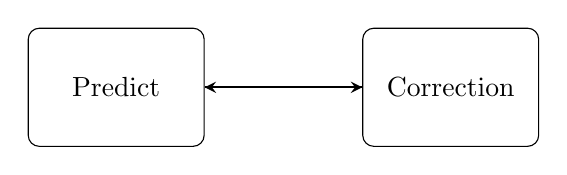
\begin{tikzpicture}[
		block/.style={rectangle, draw, text width=2cm, text centered, rounded corners, minimum height=1.5cm},
		arrow/.style={->, >=stealth, thick}
		]
		% Nodes
		\node (predict) [block] {Predict};
		\node (correct) [block, right=2cm of predict] {Correction};
		
		% Arrows
		\draw[arrow] (predict.east) -- ++(1.5cm,0) |- (correct.west) node[midway, above] {};
		\draw[arrow] (correct.west) -- ++(-1.5cm,0) |- (predict.east) node[midway, below] {};
	\end{tikzpicture}
	\caption{An Extended Kalman Filter}
	\label{kf_diagram}
\end{figure}

Prediction phase:
\[
\begin{aligned}
	\hat{x}_k^- & = f(\hat{x}_{k-1}, \bm{u}_k) \quad \text{(predicted state)}, \\
	P_k^- & = A_k P_{k-1} A_k^T + Q_k \quad \text{(predicted covariance)},
\end{aligned}
\]

where: $A_k = \frac{\partial f}{\partial x}\Bigr|_{\hat{x}_{k-1}, \bm{u}_k}$, and $Q_k$ is process noise's coveriance matrix.\\

Correction phase:
\[
\begin{aligned}
	&K_k = P_k^- H_k^T (H_k P_k^- H_k^T + R_k)^{-1} \quad \text{(Kalman's gain)}, \\
	&\hat{x}_k = \hat{x}_k^- + K_k(\bm{z}_k - h(\hat{x}_k^-)) \quad \text{(corrected state)}, \\
	&P_k = (I - K_k H_k) P_k^- \quad \text{(corrected covariance)},
\end{aligned}
\]

where: $H_k = \frac{\partial h}{\partial x}\Bigr|_{\hat{x}_k^-}$, and $R_k$ is measurement noise's covariance matrix.



\section{An Extended Kalman Filter as position and orientation estimator}

Application an Extended Kalman Filter to estimate position and orientation involves determination of state vector and state equation, specification measurement sources and their linkage with state. In prediction phase high sample rate sensors and sensor that measurements must be integrated should be used, like inertial sensor. The correction phase that can be processed rarely should include rest of sensors. In this section the filter's model will be presented.\\

In preparation, available sensors assigned into particular phase. The accelerometer and gyroscope's readings are used in prediction phase, as the reading are integrated. In correction phase external position source is used to correct position and accelerometer's readings are used to correct orientation.  Thus, the equation (\ref{u_vec}) presents the proposed control input vector and equation (\ref{h_vec}) presents measurement vector. Next state vector is set. The proposed state vector is presented in equation (\ref{state_vec}).

\begin{equation}
	\bm{u} = \begin{bmatrix}
		g_x & g_y & g_z & a_x & a_y & a_z
	\end{bmatrix}^T
	\label{u_vec}
\end{equation}

\begin{equation}
	\bm{z} = \begin{bmatrix}
		a_x & a_y & a_z & p_x & p_y & p_z
	\end{bmatrix}^T
	\label{h_vec}
\end{equation}

where:
\begin{itemize}
	\item $g_x$, $g_y$, $g_z$ -- 3 components of gyroscope's reading,
	\item $v_x$, $v_y$, $v_z$ -- 3 components of accelerometer's reading,
	\item $p_x$, $p_y$, $p_z$ -- 3 components of position from external provider.
\end{itemize}

\begin{equation}
	\bm{x} = \begin{bmatrix}
	x & y & z & v_x & v_y & v_z & q_0 & q_x & q_y & q_z & b_x & b_y & b_z & az & el
	\end{bmatrix}^T
	\label{state_vec}
\end{equation}

where:
\begin{itemize}
	\item $x$, $y$, $z$ -- 3 components of position,
	\item $v_x$, $v_y$, $v_z$ -- 3 components of velocity,
	\item $q_0$, $q_x$, $q_y$, $q_z$ -- quaternion of orientation,
	\item $b_x$, $b_y$, $b_z$ -- 3 components of gyroscope's bias,
	\item $az$ and $el$ -- azimuth and elevation of drawbar.
\end{itemize}

The bias and orientation of draw bar require an additional comment. The gyroscope's bias in state vector enable drift tracking and its compensation. Thanks to an Kalman Filter's properties the value of actual bias will be almost automatically calculated when the filter runs. The azimuth and elevation of drawbar enables utilizing external position sources even if they are not directly connected to system. In this implementation the position is given for point that is connected to system via link with fixed length. To simplify it is assumed that drawbar is connected by spherical joint to origin of moving coordinates system.\\

For the vectors so selected, the equation of state was determined. To increase readability, the state equation was split into equations (\ref{state_begin} - \ref{state_end}). The Jacobi matrix of the state function is calculated in equations (\ref{state_jacobi_begin} - \ref{state_jacobi_end}).




\begin{align}
	\bm{DCM} \left( \bm{q}_k \right) &=  \begin{bmatrix}
		q_0^2 + q_x^2 - q_y^2 - q_z^2 & 2(q_x q_y - q_0 q_z) & 2(q_x q_z + q_0 q_y) \\
		2(q_x q_y + q_0 q_z) & q_0^2 - q_x^2 + q_y^2 - q_z^2 & 2(q_y q_z - q_0 q_x) \\
		2(q_x q_z - q_0 q_y) & 2(q_y q_z + q_0 q_x) & q_0^2 - q_x^2 - q_y^2 + q_z^2 \\
	\end{bmatrix}
	\label{state_begin}
	\\
	\bm{S} \left( \bm{q}_k \right)  &= \begin{bmatrix}
		-q_x & -q_y & -q_z \\
		q_0 & -q_z & q_y \\
		q_z & q_0 & -q_x \\
		-q_y & q_x & q_0 \\
	\end{bmatrix}
	\\
	\bm{a}^W &= \bm{DCM} \left( \bm{q}_k \right) \begin{bmatrix}
		a_x \\ a_y \\ a_z 
	\end{bmatrix} - \begin{bmatrix}
		0 \\ 0 \\ g 
	\end{bmatrix}
\end{align}

\begin{align}
	\begin{bmatrix}
		x \\ y \\ z 
	\end{bmatrix}_{k+1}
	&= 
	\begin{bmatrix}
		x \\ y \\ z 
	\end{bmatrix}_{k}
	+ \Delta t
	\begin{bmatrix}
	v_x \\ v_y \\ v_z 
	\end{bmatrix}_{k}
	+ \frac{1}{2} (\Delta t)^2 \bm{a}^W
	\\
	\begin{bmatrix}
		v_x \\ v_y \\ v_z 
	\end{bmatrix}_{k+1}
	&= 
	\begin{bmatrix}
		v_x \\ v_y \\ v_z 
	\end{bmatrix}_{k}
	+ \Delta t \bm{a}^W
	\\
	\begin{bmatrix}
		q_0 \\ q_x \\ q_y \\ q_z 
	\end{bmatrix}_{k+1}
	&= 
	\begin{bmatrix}
		q_0 \\ q_x \\ q_y \\ q_z  
	\end{bmatrix}_{k}
	+ \frac{1}{2} \Delta t \bm{S} \left( \bm{q}_k \right) 
	\left(
	\begin{bmatrix}
		g_x \\ g_y \\ g_z
	\end{bmatrix}_{k}
	-
	\begin{bmatrix}
		b_x \\ b_y \\ b_z
	\end{bmatrix}_{k}
	\right)
	\\
	\begin{bmatrix}
		b_x \\ b_y \\ b_z
	\end{bmatrix}_{k+1}
	&= 
	\begin{bmatrix}
		b_x \\ b_y \\ b_z 
	\end{bmatrix}_{k}	
	\\
	\begin{bmatrix}
		az \\ el 
	\end{bmatrix}_{k+1}
	&= 
	\begin{bmatrix}
		az \\ el 
	\end{bmatrix}_{k}
	\label{state_end}
\end{align}


\begin{equation}
	\bm{D} \left( \bm{q}, \bm{a}\right)
	=
	2
	\begin{bmatrix}
		a_xq_0 + a_yq_z - a_zq_y & a_yq_0 - a_xq_z + a_zq_x & a_zq_0 + a_xq_y - a_yq_x \\
		a_xq_x + a_yq_y + a_zq_z & a_zq_0 + a_xq_y - a_yq_x & a_xq_z - a_xq_z - a_zq_x \\
		a_yq_x - a_xq_y - a_zq_0 & a_xq_x + a_yq_y + a_zq_z & a_xq_0 - a_yq_z + a_zq_y \\
		a_yq_0 - a_xq_z + a_zq_x & a_zq_y - a_yq_z - a_xq_0 & a_xq_x + a_yq_y + a_zq_z \\
	\end{bmatrix}^T
	\label{state_jacobi_begin}
\end{equation}

\begin{equation}
	\renewcommand{\arraystretch}{1.3}
	\bm{A} \left( \bm{x}, \bm{u} \right) = \frac{\partial \bm{f}}{\partial \bm{x}}
	= 
	\begin{bNiceArray}{c;c;c;c;c}
		\bm{I}_{3x3} & \Delta t \bm{I}_{3x3} & \frac{\Delta t ^2}{2}\ \bm{D} \left( \bm{q}, \bm{a}\right) & \bm{0}_{3x3} & \bm{0}_{3x2} \\
		\cdashedline
		\bm{0}_{3x3} & \bm{I}_{3x3} & \Delta t\ \bm{D} \left( \bm{q}, \bm{a}\right) & \bm{0}_{3x3} & \bm{0}_{3x2} \\
		\cdashedline
		\bm{0}_{4x3} & \bm{0}_{4x3} & \bm{I}_{4x4} & - \frac{\Delta t}{2}\ \bm{S} \left( \bm{q}_k \right) & \bm{0}_{4x2} \\
		\cdashedline
		\bm{0}_{3x3} & \bm{0}_{3x3} & \bm{0}_{3x4} & \bm{I}_{3x3} & \bm{0}_{3x2} \\
		\cdashedline
		\bm{0}_{2x3} & \bm{0}_{2x3} & \bm{0}_{2x4} & \bm{0}_{2x3} & \bm{I}_{2x2} \\	
	\end{bNiceArray}
	\label{state_jacobi_end}
\end{equation}

Next, a measurement function was determined. The accelerometer reading is used to correct orientation. The external position provider is linked with a position and drawbar orientation. The length of the drawbar is constant and equal $d$. The measurement function is given in equation (\ref{h_fun}). The Jacobi matrix of the measurement function is calculated in equations (\ref{measurement_jacobi_start} - \ref{measurement_jacobi_end}).


\begin{equation}
	\bm{h} \left(\bm{x} \right)
	= 
	\
	\begin{bmatrix}
		\bm{DCM} \left( \bm{q} \right) 
		\begin{bmatrix}
			0 \\ 0 \\ g 
		\end{bmatrix}\\
		\begin{bmatrix}
			x \\ y \\ z 
		\end{bmatrix}
		+
		\bm{R}_z \left( az \right)
		\bm{R}_y \left( el \right)
		\begin{bmatrix}
			d \\ 0 \\ 0 
		\end{bmatrix}
	\end{bmatrix}
	=
	\begin{bmatrix}
		2g(q_x q_z + q_0 q_y) \\
		2g(q_y q_z - q_0 q_x) \\
		g(q_0^2 - q_x^2 - q_y^2 + q_z^2) \\
		x + d\ cos(az)\ cos(el)\\
		y + d\ sin(az)\ cos(el)\\
		z - sin(el)
	\end{bmatrix}
	\label{h_fun}
\end{equation}

\begin{equation}
	\bm{Ca} \left( \bm{q} \right)
	=
	\begin{bmatrix}
		2q_y & 2q_z & q_0 & 2q_x \\
		-2q_x & -2q_0 & 2q_z & 2q_y \\
		2q_0 & -2q_x & -2q_y & 2q_z
	\end{bmatrix}
	\label{measurement_jacobi_start}
\end{equation}

\begin{equation}
	\bm{Cp} \left( az, el\right)
	=
	\begin{bmatrix}
		-sin(az)\ cos(el) & -cos(az)\ sin(el)\\
		 cos(az)\ cos(el) & -sin(az)\ sin(el)\\
		 0				  & -cos(el)
		
	\end{bmatrix}
\end{equation}

\begin{equation}
	\renewcommand{\arraystretch}{1.3}
	\bm{H} \left( \bm{x}, \bm{u} \right) = \frac{\partial \bm{h}}{\partial \bm{x}}
	= 
	\begin{bNiceArray}{c;c;c;c;c}
		\bm{0}_{3x3} & \bm{0}_{3x3} & g\ \bm{Ca} \left( \bm{q} \right)& \bm{0}_{3x3} & \bm{0}_{3x2} \\
		\cdashedline
		\bm{I}_{3x3} & \bm{0}_{3x3} & \bm{0}_{3x4} & \bm{0}_{3x3} & d\ \bm{Cp} \left( az, el\right) \\
	\end{bNiceArray}
	\label{measurement_jacobi_end}
\end{equation}




\section{Time synchronization problem}

Sensor's data flow to the server from multiple sensor's instance with various delays. The reading are used in prediction and correction phases. In correction phase, reading time is no so important, as this phase can be split into multiple correction. Formally, this approach is present in Multiplicative and Sequential Kalman Filters. Unfortunately, in predict phase all involved readings should be synchronized. If time of reading is known, the nearest readings are selected, or if calculation are conducted with fixed step, readings can be interpolated.\\

The time of reading is also not a trivial term, especially in decentralized system. There are many time determination method known, which differ conditions (\cite{time_sync} \cite{time_sync2}). Consider the case that assume precise clock in server and low-precision clock in every sensor node. An example method of solving the synchronization problem presents itself as follows. Every fixed period server broadcasts time synchronize message that contains only unique sequence number. Sending time $T_1$ (according to server's clock) is stored. Every node that receives synchronize message replies immediately with sequence number and node's clock time $T_n$. Received message is saved with timestamp $T_2$. Based on this reply server calculates transmission delay and clocks' offset. First transmission delay (commonly called \textit{ping}) is calculated as a half of a period between broadcasting message and receiving reply (equation (\ref{ping}))). Next, node's clock offset in respect to server's clock is calculated and stored in array (equation (\ref{offset}))). Nodes send readings signed with timestamp, that is based on node's clock. Finally, true timestamp $T_r$ in respect to server's clock is calculated by adding relevant offset (equation (\ref{timestamp}))).

\begin{equation}
	ping = \frac{T_2 - T_1}{2}
	\label{ping}
\end{equation}

\begin{equation}
	offset = T_2 - ping - T_n
	\label{offset}
\end{equation}

\begin{equation}
	T_r = T_n + offset
	\label{timestamp}
\end{equation}

\addtocontents{toc}{\protect\newpage}

\chapter{Constraints}

Constraints are the limitations imposed on the system state. They define an allowed setup, that the system can reach. Due to the origin, many types of constraints are distinguished. They can result from system's structure, known trajectory or be directly linked with limitation of mathematical instrument used in the system description.\\

A wide group of constraints is made of geometric constraints, i.e., the constraints that stem directly from the mechanism's structure. They determine the directions in which the mechanism can move so as not to breach the limits imposed by the existence of kinematic pairs.

\section{Selected constrains}

This section presents selected constraints that usually appear in robotics. Every constraint is briefly described and formulated as a function of system's state $\bm{c}(\bm{x})$ (constraint is satisfied when the function is equal to a vector of zeros). In view of its later, use a derivative of constraint function with respect to state $\frac{\partial \bm{c}(\bm{x})}{\partial \bm{x}}$ is also given.

\subsection{Quaternion norm constraint}

A quaternion is defined as four real numbers, and every coefficient is independent. However, when the quaternion is used as a description of orientation, its norm must be equal to 1. Due to the computer's precision, repetitive quaternion rotating applied in the EKF leads to error accumulation and to shrinking or stretching this norm. Moreover, the formula used in the EKF is designed to keep the constant quaternion norm only if the initial quaternion's norm had been equal to 1.\\

In mechanical simulation, this problem is solved by adding an extra pure-synthetic term to the differential equation describing the system \cite{quaternion}. Unfortunately, this method can not be easily adapted in the case of the Kalman Filter. The solution is to treat the quaternion norm equal to 1 as a constraint imposed on the system. Equation (\ref{quat_constraint_fun}) defines the constraint function, and equation (\ref{quat_constraint_fun_der}) defines its derivative. Naturally, the constraint function and its derivative are quaternion-dependent only, and they are scalar functions.

\begin{equation}
	c \left( \bm{q} \right) = \bm{q}^T \bm{q} - 1
\label{quat_constraint_fun}
\end{equation}

\begin{equation}
	\frac{\partial c}{\partial \bm{q}}  \left( \bm{q} \right) = 2\bm{q}^T
	\label{quat_constraint_fun_der}
\end{equation}

\subsection{Position and orientation constraints}

Position and orientation constraints are the constraints that are known before the system moves. They may affect only selected state variables and be applied only at certain times. The general formula that describes this type of constraint is given by equation (\ref{constraint_fun}). The derivative of this function is a mostly-zero matrix with one only on position correlated with the limited state variable.

\begin{equation}
	c \left( \bm{x} \right) = \begin{bmatrix}
		x_i - f\left(t\right) \\
		x_j - g\left(t\right)\\
		\vdots
		\end{bmatrix}
	\label{constraint_fun}
\end{equation} 

The constraints that are given by an entangled function of multiple state variables are usually harder to formulate and require an individual analysis. An example of this type is given in the next section.\\

Another example is a fixation of some parameter that can be calculated from the system state. Assume that the designed mechanism should keep the yaw angle of orientation equal to zero. If the state of the system contains orientation given by a quaternion, the yaw angle can be calculated from the following formula:

\begin{equation}
	\psi = {\mbox{atan2}}\left(2(q_{0}q_{z}+q_{x}q_{y}),1-2(q_{y}^{2}+q_{z}^{2})\right)
\end{equation}

However, the value of \textit{atan2} function is equal to zero if and only if the first argument is equal to zero. With that being said, the simple form of yaw constraint is given by equation (\ref{yaw_constraint_fun}). Equation (\ref{yaw_constraint_fun_der}) defines its derivative. The disadvantage of this approach is that the yaw angle equal to $\pi$ also fulfills the constraint.

\begin{equation}
	c \left( \bm{q} \right) = q_{0}q_{z}+q_{x}q_{y}
	\label{yaw_constraint_fun}
\end{equation}

\begin{equation}
	\frac{\partial c}{\partial \bm{q}}  \left( \bm{q} \right) =
	\begin{bmatrix}
	 q_{z} &  q_{y} &  q_{x} &  q_{0}
	\end{bmatrix}
	\label{yaw_constraint_fun_der}
\end{equation}

\subsection{Distance constraint}

The distance constraint is defined as a constraint that keeps a constant distance between a fixed point in space and a specified point on the moving element. Equation (\ref{distance_constraint_prim}) formalizes the so-defined constraint.

\begin{equation}
	\left| \bm{r}^{(0)} + R(\bm{q})\bm{s}^{(1)} - \bm{r}_p^{(0)} \right| - d = 0
	\label{distance_constraint_prim}
\end{equation}

where:
\begin{itemize}[noitemsep]
	\item $\bm{r}^{(0)}$ -- position of the moving body, given in global coordinate frame,
	\item $R(\bm{q})$ -- rotation matrix between the world frame and the body-fixed frame,
	\item $\bm{s}^{(1)}$ -- position of the selected point on the moving body, given in the body-fixed coordinate system,
	\item $\bm{r}_p^{(0)}$ -- position of the fixed point, given in the global coordinate frame,
	\item d -- the distance between constraint's points.
\end{itemize}

However, the norm of a vector requires calculation of the square root, which value and derivative are more difficult to calculate. Without any loss of generality, the distance constraint can be transformed into the following equation:

\begin{equation}
	c(\bm{r}, \bm{q}) = \left( \bm{r}^{(0)} + R(\bm{q})\bm{s}^{(1)} - \bm{r}_p^{(0)} \right)^T \left( \bm{r}^{(0)} + R(\bm{q})\bm{s}^{(1)} - \bm{r}_p^{(0)} \right) - d^2
	\label{distance_constraint_fun}
\end{equation}

In order to calculate derivative of distance constraint, the MATLAB Symbolic Toolbox was used \mbox{(\textit{distance\_constraint\_derivative.m})}. Equations (\ref{distance_constraint_der1} -- \ref{distance_constraint_der2}) presents calculated partial derivatives with respect to $\bm{r}$ and $\bm{q}$.

\begin{equation}
	\frac{\partial c(\bm{r}, \bm{q})}{r_x} = 2(x - r_{bx} + r_{ax}(2q_0^2 + 2q_x^2 - 1) + r_{ay}(2q_0q_z - 2q_xq_y) + r_{az}(2q_0q_y - 2q_xq_z))^2 
	\label{distance_constraint_der1}
\end{equation}

\begin{equation}
	\frac{\partial c(\bm{r}, \bm{q})}{r_y} = 2(y - r_{by} + r_{ay}(2q_0^2 + 2q_y^2 - 1) + r_{ax}(2q_0q_z + 2q_xq_y) + r_{az}(2q_0q_x + 2q_yq_z))^2
\end{equation}

\begin{equation}
	\frac{\partial c(\bm{r}, \bm{q})}{r_z} = 2(z - r_{bz} + r_{az}(2q_0^2 + 2q_z^2 - 1) + r_{ax}(2q_0q_y + 2q_xq_z) - r_{ay}(2q_0q_x - 2q_yq_z))^2
\end{equation}

\begin{align}
\begin{split}
	\frac{\partial c(\bm{r}, \bm{q})}{q_0} &= 2(2q_yr_{az} - 4q_0r_{ax} + 2q_zr_{ay})(r_{bx} - x - r_{ax}(2q_0^2 + 2q_x^2 - 1)\\
	&+ r_{ay}(2q_0q_z - 2q_xq_y) + r_{az}(2q_0q_y - 2q_xq_z))^2\\
	&+ 2(4q_0r_{ay} +  2q_xr_{az} + 2q_zr_{ax}) \cdot(y - r_{by} + r_{ay}(2q_0^2 + 2q_y^2 - 1)\\
	&+ r_{ax}(2q_0q_z + 2q_xq_y) + r_{az}(2q_0q_x + 2q_yq_z))^2 + 2(4q_0r_{az} - 2q_xr_{ay} + 2q_yr_{ax})\\
	&\cdot(z - r_{bz} + r_{az}(2q_0^2 + 2q_z^2 - 1) + r_{ax}(2q_0q_y + 2q_xq_z) - r_{ay}(2q_0q_x - 2q_yq_z))^2
\end{split}
\end{align}

\begin{align}
\begin{split}
	\frac{\partial c(\bm{r}, \bm{q})}{q_x} &= 2(2q_0r_{az} + 2q_yr_{ax})(y - r_{by} + r_{ay}(2q_0^2 + 2q_y^2 - 1)\\
	&+ r_{ax}(2q_0q_z + 2q_xq_y) + r_{az}(2q_0q_x + 2q_yq_z))^2\\
	&- 2(4q_xr_{ax} + 2q_yr_{ay} + 2q_zr_{az})(r_{bx} - x - r_{ax}(2q_0^2 + 2q_x^2 - 1)\\
	&+ r_{ay}(2q_0q_z - 2q_xq_y) + r_{az}(2q_0q_y - 2q_xq_z))^2 - 2(2q_0r_{ay} - 2q_zr_{ax})\\
	&\cdot(z - r_{bz} + r_{az}(2q_0^2 + 2q_z^2 - 1) + r_{ax}(2q_0q_y + 2q_xq_z) - r_{ay}(2q_0q_x - 2q_yq_z))^2
\end{split}
\end{align}

\begin{align}
	\begin{split}
	\frac{\partial c(\bm{r}, \bm{q})}{q_y} &= 2(2q_xr_{ax} + 4q_yr_{ay} + 2q_zr_{az})(y - r_{by} + r_{ay}(2q_0^2 + 2q_y^2 - 1)\\
	&+ r_{ax}(2q_0q_z + 2q_xq_y) + r_{az}(2q_0q_x + 2q_yq_z))^2\\
	&+ 2(2q_0r_{az} - 2q_xr_{ay})(r_{bx} - x - r_{ax}(2q_0^2 + 2q_x^2 - 1) \\
	&+ r_{ay}(2q_0q_z - 2q_xq_y) + r_{az}(2q_0q_y - 2q_xq_z))^2 + 2(2q_0r_{ax} + 2q_zr_{ay})\\
	&\cdot(z - r_{bz} + r_{az}(2q_0^2 + 2q_z^2 - 1) + r_{ax}(2q_0q_y + 2q_xq_z) - r_{ay}(2q_0q_x - 2q_yq_z))^2
\end{split}
\end{align}

\begin{align}
	\begin{split}
	\frac{\partial c(\bm{r}, \bm{q})}{q_z} &= 2(2q_xr_{ax} + 2q_yr_{ay} + 4q_zr_{az})(z - r_{bz} + r_{az}(2q_0^2 + 2q_z^2 - 1)\\
	&+ r_{ax}(2q_0q_y + 2q_xq_z) - r_{ay}(2q_0q_x - 2q_yq_z))^2\\
	&+ 2(2q_0r_{ay} + 2q_xr_{ax})(r_{bx} - x - r_{ax}(2q_0^2 + 2q_x^2 - 1)\\
	&+ r_{ay}(2q_0q_z - 2q_xq_y) + r_{az}(2q_0q_y - 2q_xq_z))^2 - 2(2q_0r_{ax} - 2q_yr_{ay})\\
	&\cdot(y - r_{by} + r_{ay}(2q_0^2 + 2q_y^2 - 1) + r_{ax}(2q_0q_z + 2q_xq_y) + r_{az}(2q_0q_x + 2q_yq_z))^2
	\label{distance_constraint_der2}
\end{split}
\end{align}
\\

It is worth mentioning that if velocities are known, the equation function (\ref{distance_constraint_fun}) can be differentiated with respect to time to get extra constraint $c(\bm{r}, \bm{q}, \frac{d\bm{r}}{dt}, \frac{d\bm{q}}{dt})$. Nevertheless, the position and velocity are strictly connected within the EKF state function. As a result, the correction of position leads to the correction of velocity.


\section{Inclusion of constraints in the estimation}

Assume that a novel system for locating metro wagons is planned to be developed. The first idea that comes to mind is to use a satellite navigation system, as is usually the case in location-based tasks. However, this solution suffers from a significant flaw: these systems perform much worse underground. The question is whether the quality of the position estimate can be easily improved, and the short answer is yes. A simple assumption that can be made is that metro wagons can only be on the rails. Using the well-known track, it is possible to stick the calculated location to the nearest rails, thus improving its accuracy.
This illustrative example implicitly demonstrates the principle of constraint's correction.\\

The inclusion of constraints in state estimation is not a popular solution. Usually, transform to other state variables that fulfill constraints is suggested. However, it provokes the redesign of the state estimator every time when constraints change. The unique approach is discussed by Dan Simon in articles \cite{simon}, \cite{simon2010kalman} and \cite{simon2006kalman}. It is proposed to add the third phase to the conventional Extended Kalman Filter, as it is shown in figure \ref{ekf_three_phases}.

\begin{figure}[!h]
	\begin{center}
		\begin{tikzpicture}[
			block/.style={rectangle, draw, text width=2cm, text centered, rounded corners, minimum height=1.5cm},
			arrow/.style={->, >=stealth, thick},
			>=Stealth,
			]
			% Nodes
			\node (predict) [block] {Prediction};
			\node (correct) [block, right=3cm of predict] {Correction};
			\node (constraints) [block, below left=0.5cm and 0.33cm of correct] {Constraints};
			
			% Arrows
			\draw[bend left=20,-latex] ($(predict.east)+(0,0.3)$) to ($(correct.west)+(0,0.3)$);
			\draw[bend left=40,-latex] (correct.south) to (constraints.east);
			\draw[bend left=40,-latex] (constraints.west) to (predict.south);
			
		\end{tikzpicture}
	\end{center}
	\caption{Stages in the Extended Kalman Filter with constraint correction}
	\label{ekf_three_phases}
\end{figure}

In the constraints correction phase, only the state of the filter changes, and the covariance matrix remains unchanged. For linear constraints $\left( \bm{D} \bm{x} = \bm{d}  \right)$, the following equation presents constraints correction phase:

\begin{equation}
	\bm{\tilde{x}} = \bm{\hat{x}} - \bm{W}^{-1} \bm{D}^T \left( \bm{D} \bm{W}^{-1} \bm{D}^T \right)^{-1} \left( \bm{D} \bm{\hat{x}} - \bm{d}  \right)
	\label{constraint_corr}
\end{equation}

where:
\begin{itemize}[noitemsep]
	\item $\bm{D}$, $\bm{d}$ -- matrix and vector defining linear constraints,
	\item $\bm{W}$ -- square weight matrix,
	\item $\bm{\hat{x}}$ -- filter state before correction,
	\item $\bm{\tilde{x}}$ -- filter state after correction.
\end{itemize}

It is proposed to use the inverse of covariance matrix as the weight matrix  $\bm{W} = \bm{P}^{-1}$. In the case of linear constraints, it leads to the maximum probability
estimate of the state subject to state constraints.\\

Proof of the correctness of this method is well-known in the literature. So as not to duplicate this, another proof will be presented by showing the similarity to Newton-Raphson's nonlinear equations solving method. Assume that $\bm{D}$ is a square matrix with full rank. In order to find the solution of constraint equations, an iterative method is used to solve equation (\ref{Dxd}). The Newton-Rapshon method requires the Jacobi matrix, which in this case is given in equation (\ref{D})

\begin{equation}
	\bm{f} \left( \bm{x} \right) = \left( \bm{D} \bm{x} - \bm{d}  \right)
	\label{Dxd}
\end{equation}

\begin{equation}
	\frac{\partial \bm{f} \left( \bm{x} \right)}{\partial \bm{x}} = \bm{D}
	\label{D}
\end{equation}

According to the Newton-Raphson method, every iteration is given by:
\begin{equation}
	\bm{\tilde{x}} = \bm{\hat{x}} - \left( \frac{\partial \bm{f} \left( \bm{x} \right)}{\partial \bm{x}} \right) ^{-1} \bm{f} \left( \bm{x} \right) = \bm{\hat{x}} - \bm{D}^{-1} \left( \bm{D} \bm{\hat{x}} - \bm{d}  \right)
	\label{NR}
\end{equation}

In general $\bm{D}$ matrix is not square, as there is fewer constraints than the degree of freedom of the mechanisms and $\bm{D}$ can not be inverse trivial. To address this problem right pseudo-inverse can be used (equation (\ref{pseudoinverse})).
\begin{equation}
	\bm{D}^{\#} = \bm{D}^T \left( \bm{D} \bm{D}^T \right) ^ {-1}
	\label{pseudoinverse}
\end{equation}

Furthermore, if the equation is underdetermined, the pseudo-inverse forms a space of proper inverses, scaled by a weight matrix $\bm{W}$:

\begin{equation}
	\bm{D}^{\#} = \bm{W}^{-1} \bm{D}^T \left( \bm{D} \bm{W}^{-1} \bm{D}^T \right) ^ {-1}
	\label{wieight_pseudo}
\end{equation}

Inserting equation (\ref{wieight_pseudo}) to (\ref{NR}) leads to the constraint correction equation (\ref{constraint_corr}).\\

It is worth mentioning that the presented method of calculating the pseudoinverse of D is only valid under the assumption of a full order of the D matrix. The reduction of the order of the matrix occurs when the constraints become linearly dependent. In this situation, another method of calculating pseudo-inversion should be used, e.g, SVD decomposition. \cite{golub2013matrix}\\

The reasoning so far was based on the assumption that constraints are linear. 
However, constraints in mechanics are mostly nonlinear. This problem is addressed by the local linearization method. The following equation define substitutions resulting from linearization:

\begin{equation}
	\bm{D} = \frac{\partial \bm{c}}{\partial \bm{x}}(\bm{\hat{x}})
	\label{linearization1}
\end{equation}

\begin{equation}
	\bm{d} =  - \bm{c} (\bm{\hat{x}}) +  \frac{\partial \bm{c}}{\partial \bm{x}}(\bm{\hat{x}}) \bm{\hat{x}}
	\label{linearization2}
\end{equation}

As a result, the constraint correction method can be used for nonlinear equations.\\ 

Direct application of the method to the discussed problem proved not to work properly and led to instability. However, some improvements were introduced based on the analogy of the constraint correction method to the Newton-Raphson method. The idea behind the proposed enhancement is to divide the correction into many smaller steps. It is proposed to use an additional coefficient $\alpha$ that scales the correction term. By design, the coefficient should be within the range $(0, 1 \rangle $. Next, as the impact of correction was reduced by scaling, it is proposed to conduct the correction multiple times within one run of this phase. This is analogous to the iterations performed by the Newton-Raphson method. The following formula presents the improved constraint correction method with k-times repetition:

\begin{equation}
	\bm{\hat{x}}_{i+1} = \bm{\hat{x}}_{i} - \alpha \bm{P} \bm{D}^T \left( \bm{D} \bm{P} \bm{D}^T \right)^{-1} \left( \bm{D} \bm{\hat{x}} - \bm{d}  \right) \hspace{10pt} \text{for i = 1,2,..,k}
	\label{constraint_final}
\end{equation}

The selection of newly introduced parameters belongs to the tuning, and the correctness and usefulness of the proposed enhancement have been corroborated experimentally.

\chapter{Designed system}

\section{Specification}

Based on the knowledge gathered, the functional requirements for the system were formulated and described using use case methodology, where system is an actor.

System:
\begin{itemize}
	\item uses inerial sensor the measure accelerations and angular velocities,
	\item retrieves data from external sensor and data providers,
	\item filters raw data,
	\item conduct sensor fusion to estimate position and orientation,
	\item store readings and estimations in files,
	\item displays system's state for operator.
\end{itemize}

Beside above requirement, also non-functional requirements were formed. Table (\ref{furps}) presents requirements using FURPS metodology.

\section{System architecture}

The system is organized into modules. The individual modules perform the following tasks:\\

\noindent\textbf{server} -- central module processing and storing data. Performs raw data filtration, sensor fusion and saving logs. Communicate with sensors and provides system's time. Issues the API used by the front-end application.\\

\noindent\textbf{node\_udp} -- sensor node's source code. Performs raw data collecting and efficient forwarding to server. Due to abstraction layer software is highly independent of  node's hardware.\\

\noindent\textbf{client} -- front-end application to visualize system's status and control it. Ultimately constitutes the main human-machine interface.\\

\noindent\textbf{constraints} -- library providing constraints' equations. Separates mechanical structure from server source code.\\

\noindent\textbf{bridge} -- sensor node's mock, intended as rapid prototyping tool. Connects to server via same protocol as node\_udp.\\

\noindent\textbf{docker} -- Docker container's configuration. Container wraps the server and makes it independent of host machine. Prepared image can be run on every Docker-compatible machine.\\

Figure (\ref{architecture}) shows system architecture's diagram with communication paths between modules.

\begin{figure}[!h]
	\begin{center}
		\begin{tikzpicture}[
			block/.style={rectangle, draw, text width=2cm, text centered, rounded corners, minimum height=1.5cm},
			arrow/.style={<->, >=stealth, thick},>=Stealth,
			]
			% Nodes
			\node (server) [block, minimum width = 5cm, minimum height = 5cm] {Server};
			\node (node) [block, above left=0.6cm and 5cm of predict] {Node UDP};
			\node (bridge) [block, above left=-1.2cm and 5cm of predict] {Bridge};
			\node (client) [block, right=5cm of predict] {Client};
			\node (constraints) [block, below right=-1.8cm and -2.5cm of server] {Constraints};
			\node (docker) [block, minimum width = 6cm, minimum height = 7cm] {};
			\node [below right] at (docker.north west) {Docker};
			\node (ext) [block, below left=0.6cm and 5cm of predict] {External sources};
			
			% Arrows
			\draw[arrow] (server.east)  -- (client.west) node[midway, above] {ZeroMQ (TCP)};
			\draw[arrow] (server.west|-node.east)  -- (node.east) node[midway, above] {UDP};
			\draw[arrow] (server.west|-bridge.east)  -- (bridge.east) node[midway, above] {UDP};
			\draw[arrow] (server.west|-ext.east)  -- (ext.east) node[midway, above] {TCP/UDP};
			
		\end{tikzpicture}
	\end{center}
	\caption{System architecture's diagram}
	\label{architecture}
\end{figure}

\section{Technologies}

The implementation of the project used various software technologies and libraries. The following summary explains the choice of specific technologies.\\

\noindent\textbf{server, constraints} -- due to the large computational effort required to run online calculations, the C++ language was chosen. Because of its performance and flexibility, it is a natural choice for efficient computer simulations. In addition, the following libraries were used:
\begin{itemize}[noitemsep,nolistsep]
	\item Eigen3 -- a library containing elements of linear algebra: matrices, vectors and related algorithms. Eigen3 prioritizes efficiency by using SIMD and maintains a clear syntax.
	\item ZeroMQ -- libzmq library binding for C++. Libzmq is a base implementation of ZeroMQ queues written in C,
	\item yaml-cpp -- a library providing YAML serializer and deserializer,
	\item Boost -- multi-purpose C++ library, in case of this project Boost provides asynchronous TCP and UDP client. 
	\item libmodbus -- a library providing support for MODBUS protocol
\end{itemize}
\  \\
\textbf{node\_udp} -- embedded source code is also written in C++, due to the fact that microcontroller's producers usually provides a base chip's API using C or C++. C++ is currently the first choice language for Atmega, STM and ESP chips.\\

\noindent\textbf{client} -- having in mind the provision of cross-platform, the Qt library was used to implement the front-end application. Further, to avoid multiple compilation Python Qt library was used. \\

\noindent\textbf{bridge} -- the implementation also uses Python, but due to its other features. Bridge is supposed to be rapid developed, and its code should be understood for as many developers as possible,\\

\noindent\textbf{docker} -- as the name suggests, Docker was used to containerize system.   
	
\section{Prototype}
Project realization includes the preparation of software and hardware. The hardware part is the sensor node, that perform low-lever sensor data collecting and transferring data to server. The selected hardware should provide adequate performance and support network communication. For this purpose, microcontrollers work well. Wemos D1 mini Pro development board was selected. The ESP8266EX chip used on it provides high performance and native support for network functions including Wi-Fi. Board is connected to two shields: power supply shield and custom shield with IMU. Power supply shield enables chip powering from Li-ion battery. Custom shield has installed Pololu MinIMU-9 that contains LSM303 accelerometer and L3GD20 gyroscope. Thus created device is very compact and together with battery fits into a 50x40x35mm 3D-printed enclosure (figure (\ref{prototype})).

\begin{figure}[!h]
	\begin{center}
		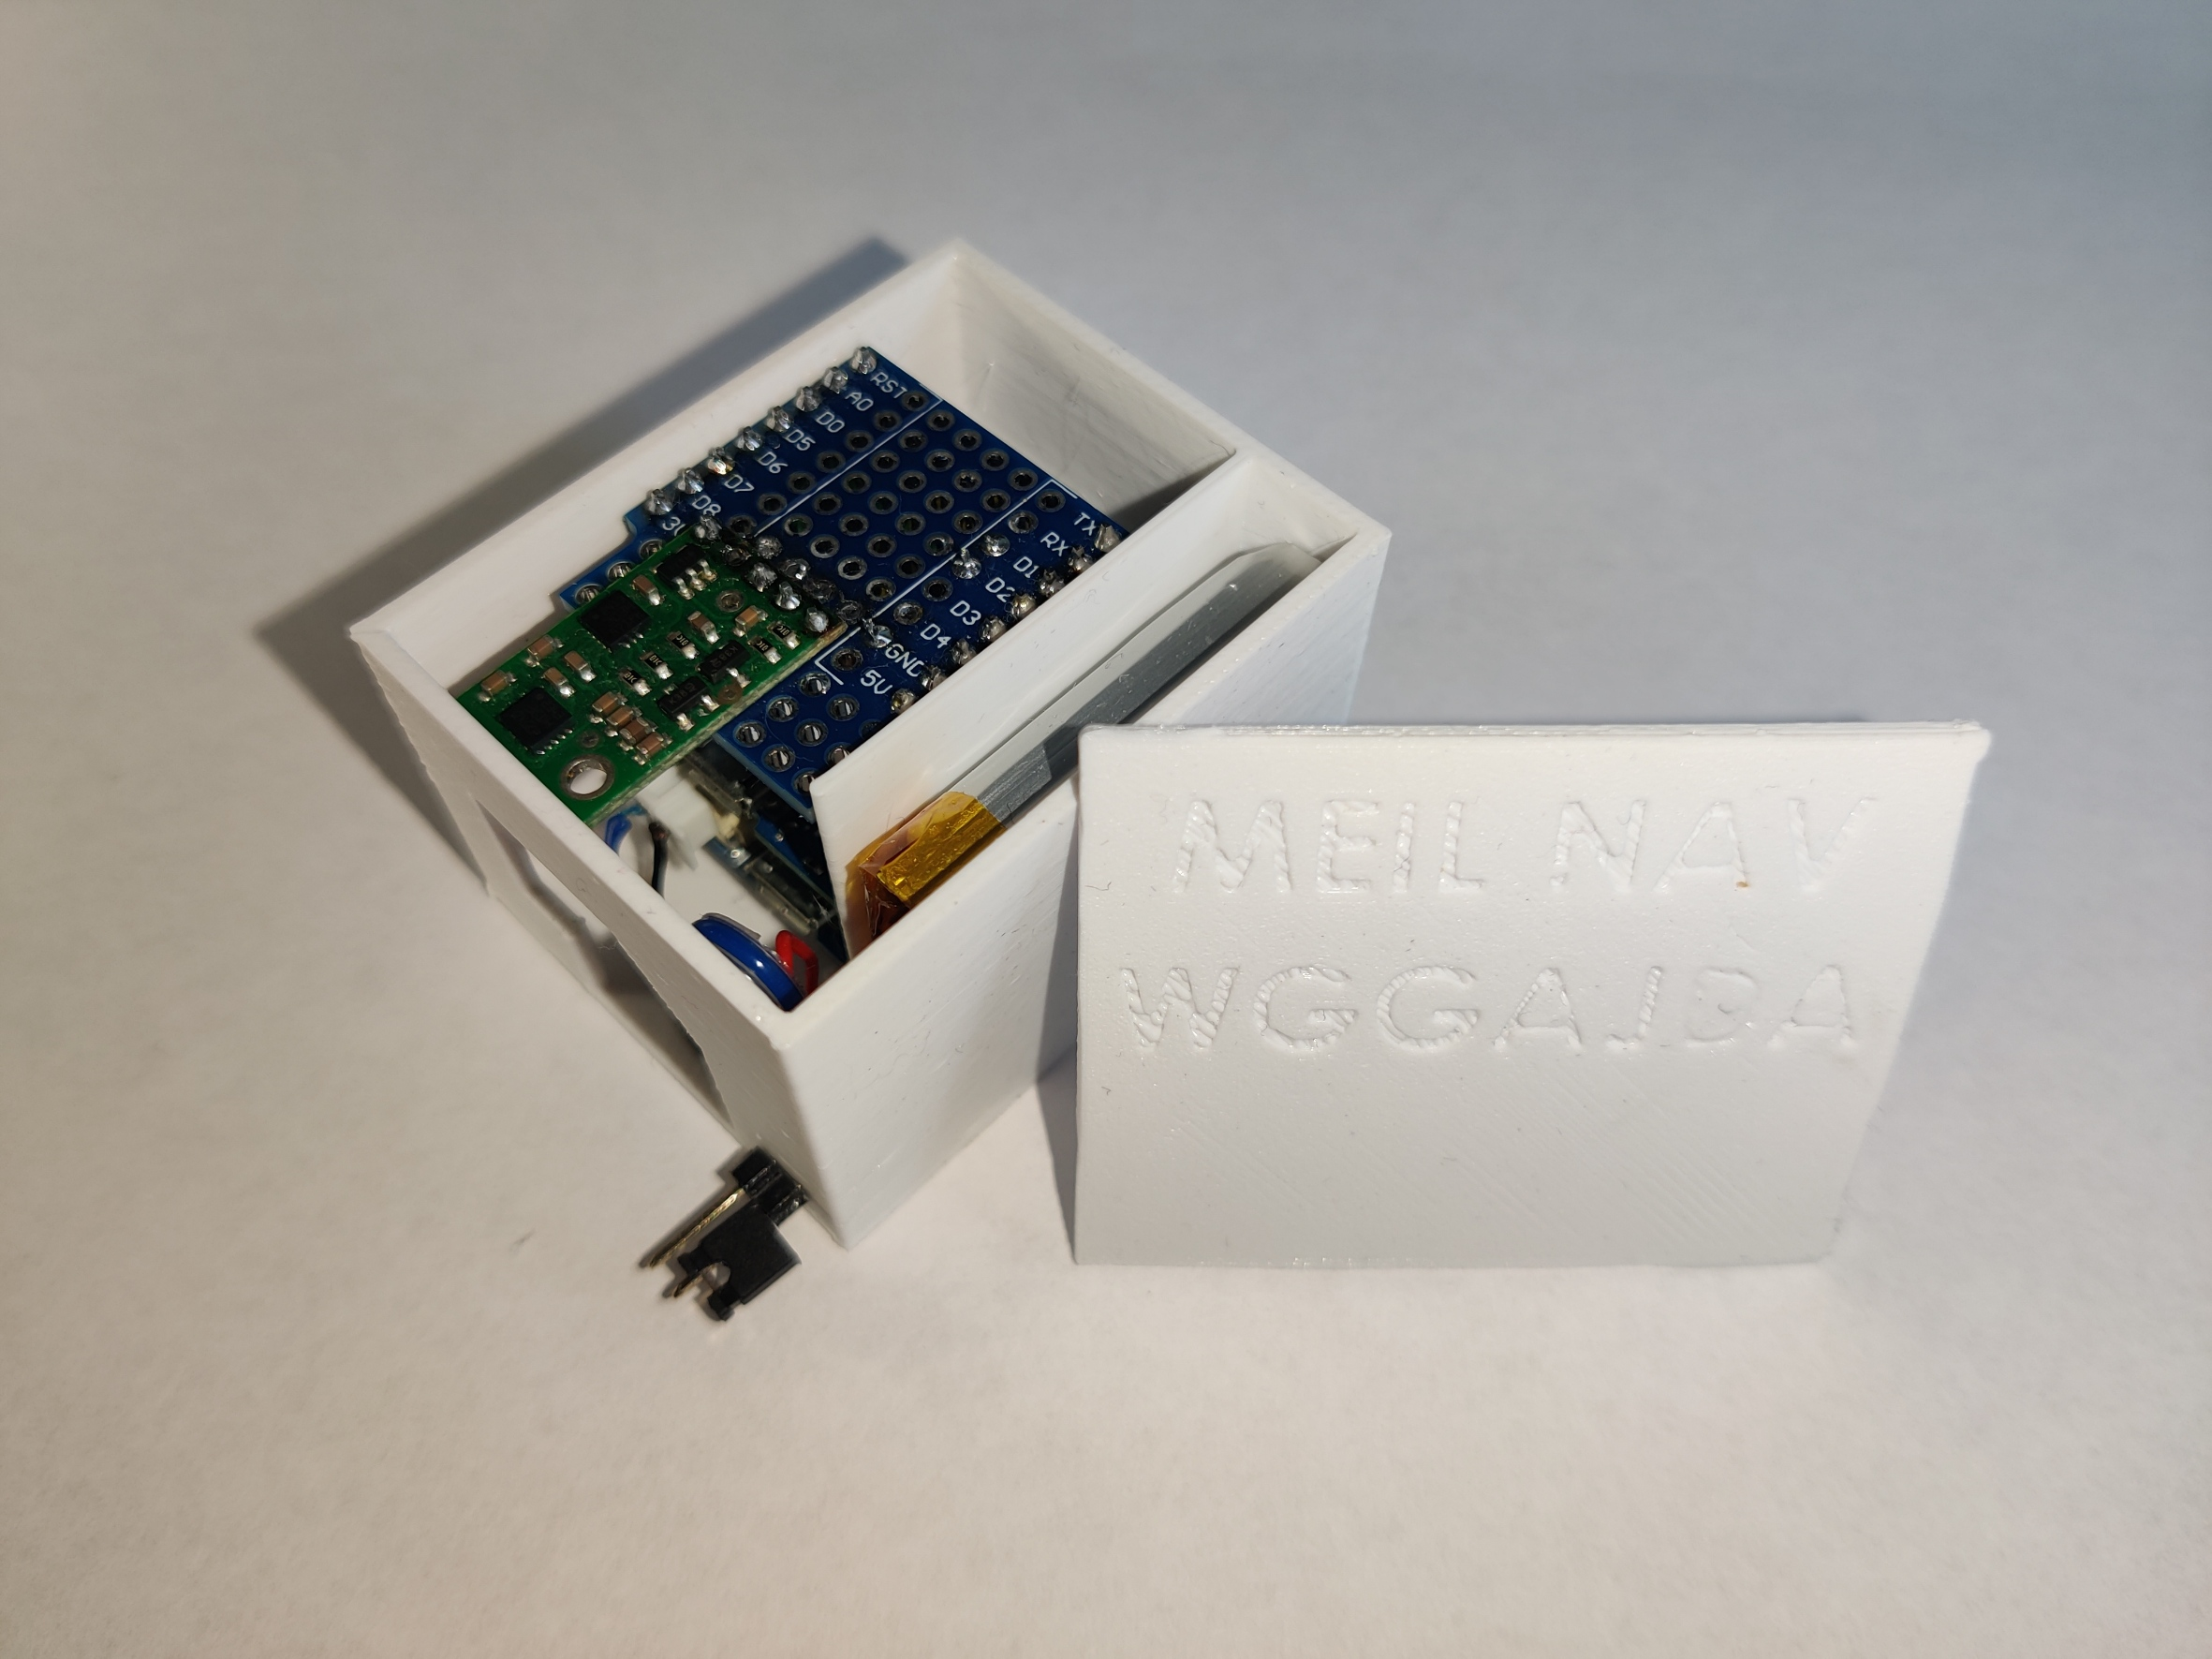
\includegraphics[width = 0.8\textwidth]{prototype.jpg}
	\end{center}
	\caption{Sensor node}
	\label{prototype}
\end{figure}

\renewcommand{\arraystretch}{1.2}
\begin{table}[!h]
	\centering
	\begin{tabular}{|m{0.03\textwidth}|m{0.13\textwidth}|m{0.025\textwidth}|m{0.68\textwidth}|} 
		\hline
		\rowcolor{Gray}		\multicolumn{2}{|c|}{Requirement} & No. & Description \\
		\hline
		\centering \multirow{2.0}{*}{\rotatebox[origin=c]{90}{Usability}}
		&\multirow{1}{*}{Usability} 
		& 1 & Server runs natively on UNIX or in Docker containter. Front-end application is multi-platform. \\
		\cline{2-4}
		& \multirow{1}{*}{Ergonomy} 
		& 2 & User interface should be transparent and intuitive.  \\
		\cline{3-4}
		\hline
		\centering \multirow{2.0}{*}{\rotatebox[origin=c]{90}{Reliability}}
		& \multirow{1}{*}{Precision} 
		& 3 & System should maximize estimation precision for collected readings. \\
		\cline{2-4}
		& \multirow{1}{*}{Verifiability} 
		& 4 & Estimation results should match predictions and be verifiable. \\
		\hline
		\centering \multirow{1}{*}{\rotatebox[origin=c]{90}{Perf.}}
		& \multirow{1}{*}{Performance} 
		& 5 & System performance should scale relative to number of sensors. \\
		\hline
		\centering \multirow{5.5}{*}{\rotatebox[origin=c]{90}{Supportability}}
		& \multirow{2}{*}{Maintenance} 
		& 6 & System implementation should be transparent and easy to develop.  \\
		\cline{3-4}
		& & 7 & System should be divided into modules, that can be modified separately.\\
		\cline{2-4}
		& \multirow{1}{*}{Installability} 
		& 8 & Installation process should be easy. It is recommanded for front-end software not to be installed. \\
		\cline{2-4}
		& \multirow{1}{*}{Configuration} 
		& 9 & Software should be magic-number-free and all parameters should be configurable. \\
		\hline
	\end{tabular}
	\caption{Non-functional requirements -- FURPS}
	\label{furps}
\end{table}

\section{Plugins}

The developed software creates an advanced multitask system. During its preparation there was a lot of attention paid to make software flexible and easily updated. This allows you to enrich the system with features needed for specific applications. Those addons, that are not strictly connected with system's main task are called plugin.\\

An example of plugin, that was added to system is force logger. The main task of this plugin is collecting data from tension transducer connected via MODBUS TCP. For this purpose force logger utilizes already implemented timestamp system and save logs in project's specific format. Stored data are also synchronized with other estimations.

\section{Tuning}

Tuning is a process selection of a set of parameters provides the best results in terms of the chosen criterion. For the solution being developed, the greatest number of unknowns are the parameters of sensor filtration and fusion. Based on similar projects and applications, the initial value of parameters can be selected, but the tuning is an unmissable step on the way to precise estimation.\\

In measurement systems, the final result is affected by almost every element of the system: sensor errors, installation errors, delays and more. Due to that, there is no universal method of tuning. The process largely depends on the operator's experience and ability to recognize system responses. Nevertheless, it is prolific to plan the experiments that highlight certain regions of interest and, as a result, lead to shorter tuning times.\\

The project took care to include all the parameters in a configuration file that is freely editable. Parameters were divided into categories and a few of them can be modified on-line, when the system runs. The source code is devoid of modifiable numerical constants (so-called \textit{magic numbers}). Additionally, the configuration file contains software variables that define network topology, addressing and other parameters that are configured during deployment.



\chapter{Case study}


Case study describes a solution's deployment on the mechanism that was a motivation for this project. The mechanism shown on figures (\ref{fig:mbs} - \ref{fig:render}) is an overconstrainted multibody system (\cite{bib:BPAS2012}), that involves moving platform connected to ground by 6 rigid rods. The lower and upper rods are parallel to each other and have equal length. Although constraints describing the mechanism form a six-dimensional system of equations, they are linear dependent what is observable as a movement of the platform. The mechanism has one degree of freedom, except for two points where a bifurcation occurs. Due to this anomaly it's hard to simplify mechanism model to minimal set of coordinates.

\begin{figure}[!h]
	\centering
	\begin{minipage}{.5\textwidth}
		\centering
		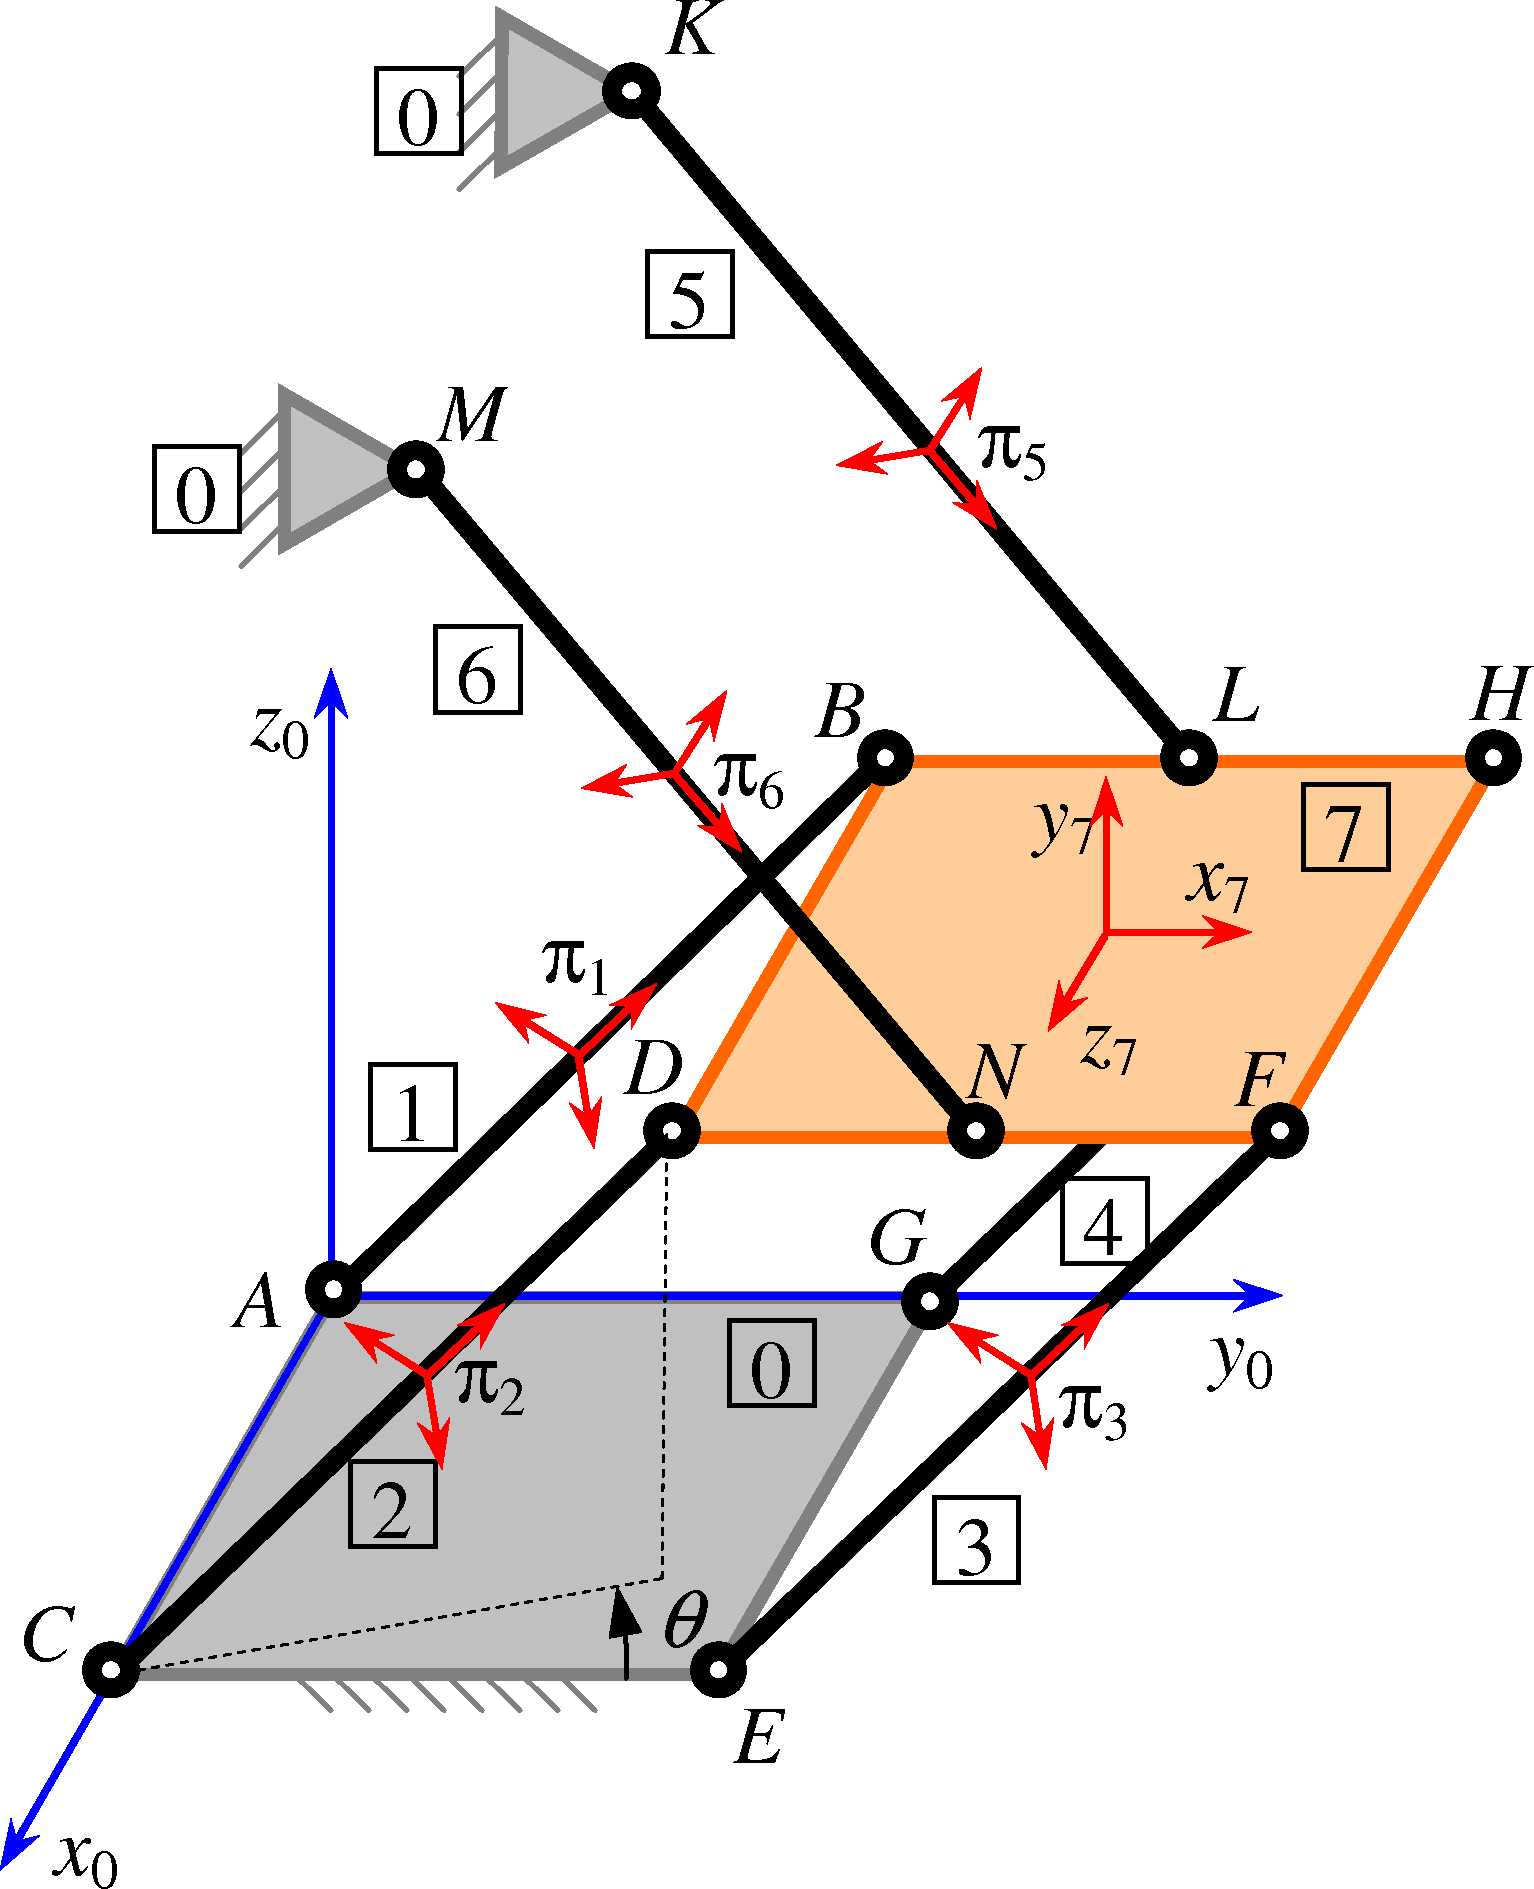
\includegraphics[width=.7\linewidth]{mbs_system.png}
		\captionof{figure}{Multi-body system with 1 DOF}
		\label{fig:mbs}
	\end{minipage}%
	\begin{minipage}{.5\textwidth}
		\centering
		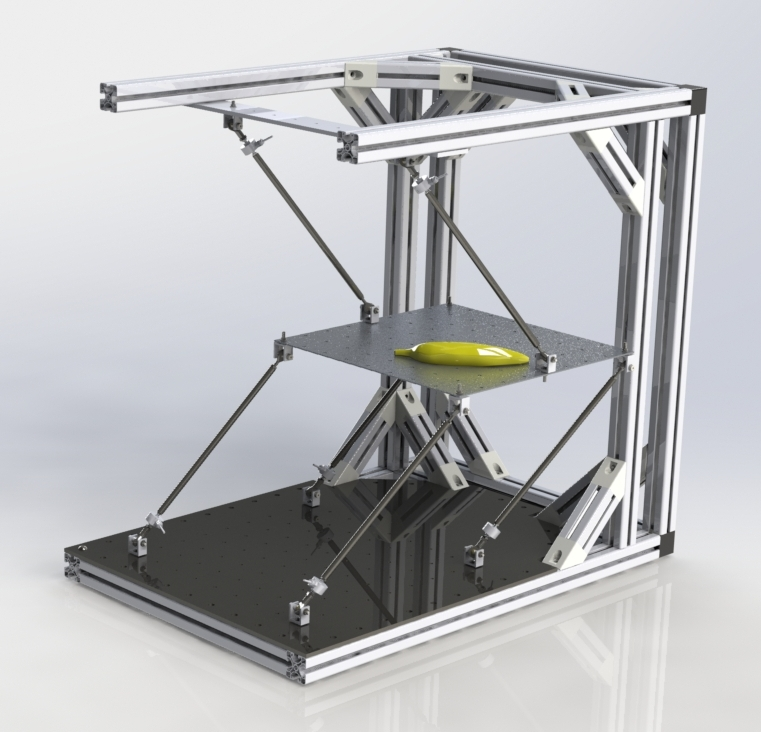
\includegraphics[width=.9\linewidth]{render.jpg}
		\captionof{figure}{Render of the MBS}
		\label{fig:render}
	\end{minipage}
\end{figure}

The scientific significance of this mechanism is revealed in the determination of the reaction forces that occur in rods. Mechanism is statically indeterminate which makes it even more difficult to analyze and highlights its research value. The further researches require collecting data from test stand, when the platform moves. State description should contain platform's position and orientation as well as readings from force sensor installed in rods, what is covered by developed system.\\

The mechanism is driven by FANUC M-10iA serial industrial robots. The robot's control system provides arm's tip position. To avoid problems resulting from inaccurate manufacturing the robot is connected to platform center via a drawbar, so the tip's orientation is unusable. Moreover, the position's refresh rate is relatively slow, but can be successfully used in sensor fusion.\\

The mechanism thus presented is a representative example of the application of the developed measuring system. Due to its properties, conventional methods are hard to apply. The proposed solution is challenging as well, but the procedure that leads to a working system is structured and split into steps. 

\section{Computer simulation}

Before real-life experiments, the fundamental aspects of projected were tested in computer simulation. The simulation involves preparing kinematic simulation in ADAMS and connecting it with simplified estimation system in MATLAB Simulink. A finished model was used, created earlier as part of a research project. The ADAMS's model was extended with new cylinder-shaped body that represents the robot's tip. The added part is connected with the moving platform's center and will be used as a motion source. A position of the simulated robot's tip is set as a control variable, that input to the program. The kinematic's simulation's outputs are postion and orientation of the moving platform, and its linear acceleration and angular velocity expressed in local coordinates system. Those variables will be used to simulate sensors' readings.
A figure (\ref{adams}) presents multi-body system modeled in ADAMS software. Thus prepared model was converted to a Simulink block. 

\begin{figure}[!h]
	\centering
	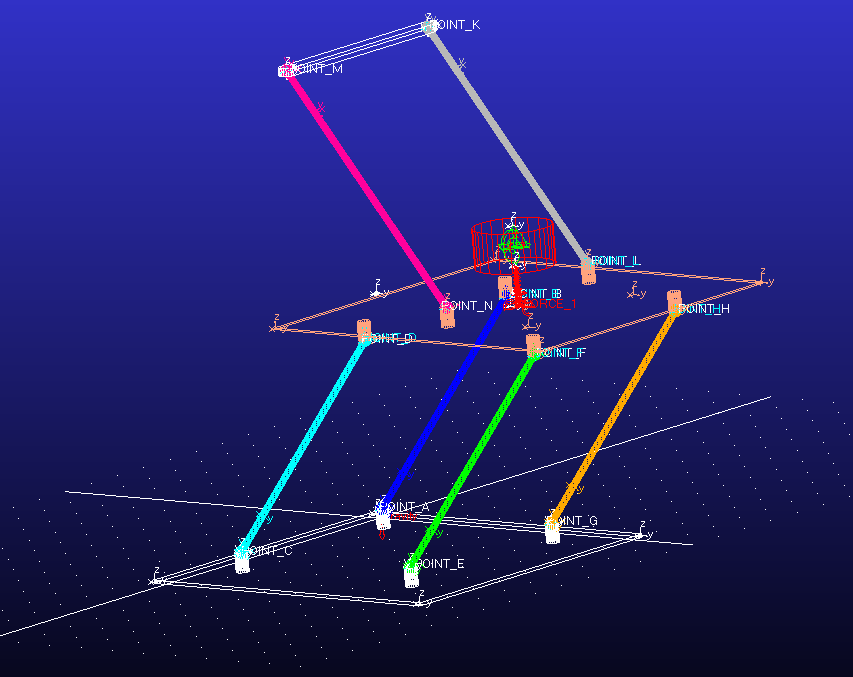
\includegraphics[width=0.8\textwidth]{duw/adams.png}
	\caption{The mechanism modeled in ADAMS software}
	\label{adams}
\end{figure}

Next, to move the mechanism, a trajectory generator was prepared. One of the allowed trajectories is a circular motion in the horizontal plane. In order to check position tracking, the tangential velocity was constantly increased. Equations (\ref{tcp_begin} - \ref{tcp_end}) present the three components of the robot's tip as a function of time.

\begin{align}
	x_{TCP} &= x_0 +  R\ cos( t^2 )
	\label{tcp_begin}\\
	y_{TCP} &= y_0  + R\ sin( t^2 )\\
	z_{TCP} &= z_0
	\label{tcp_end}
\end{align}

With the platform that already moves, the following stage is to simulate inertial sensors: an accelerometer and a gyroscope. The sensors are simulated based on ADAMS block outputs. The gyroscope returns an angular velocity, while the accelerometer returns linear velocity with gravitation acceleration added. Figure \ref{acc_sym} presents Simulink blocks that represent an ideal accelerometer.

\begin{figure}[!h]
	\centering
	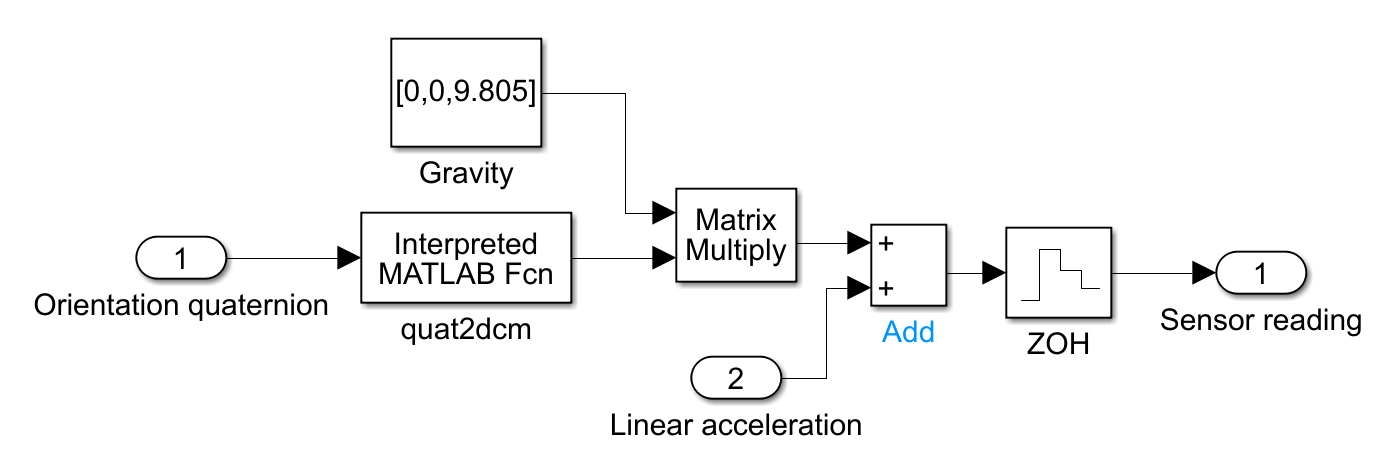
\includegraphics[width=0.7\textwidth]{duw/acc_sim.png}
	\caption{The simulation of an accelerometer}
	\label{acc_sym}
\end{figure}

The outputs of ideal sensors' simulation are further passed to blocks that represents sensor's error. In this simplified simulation the sensor's error was limited to adding a pink noise and bias. A figure (\ref{error_sensor}) presents Simulink blocks that represents a sensor's error.

\begin{figure}[!h]
	\centering
	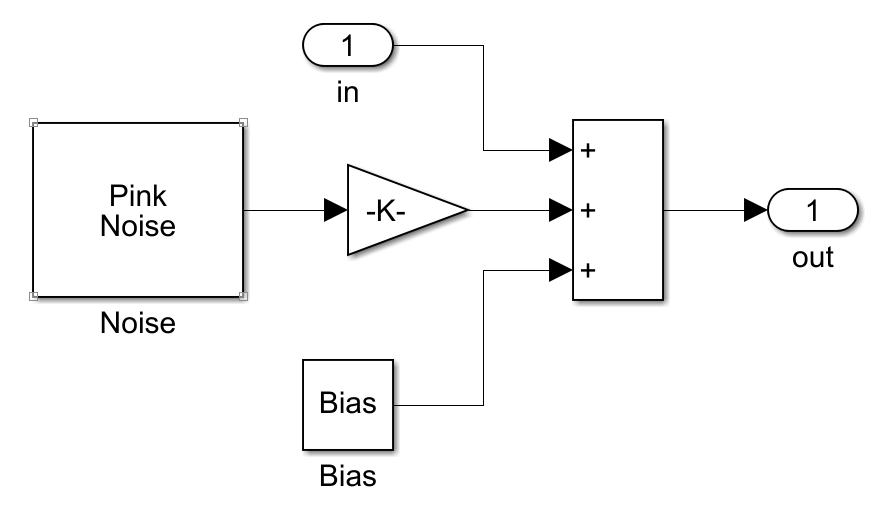
\includegraphics[width=0.7\textwidth]{duw/error.png}
	\caption{The simulation of a sensor error}
	\label{error_sensor}
\end{figure}

The final step was to implement and tune the Kalman Filter with constraints' correction. Once again, the MATLAB implementation is a simplified version of the filter described in section (\ref{filter_model}). An implemented constraints are given in equations (\ref{simplified_eq} -- \ref{simplified_eq2}).  A figure (\ref{ekf_sim}) presents the realization of filter in Simulink MATLAB.

\begin{align}
	x^2 + y^2 - r^2 &= 0
	\label{simplified_eq}\\
	z &= 0
	\label{simplified_eq2}
\end{align}

\begin{figure}[!h]
	\centering
	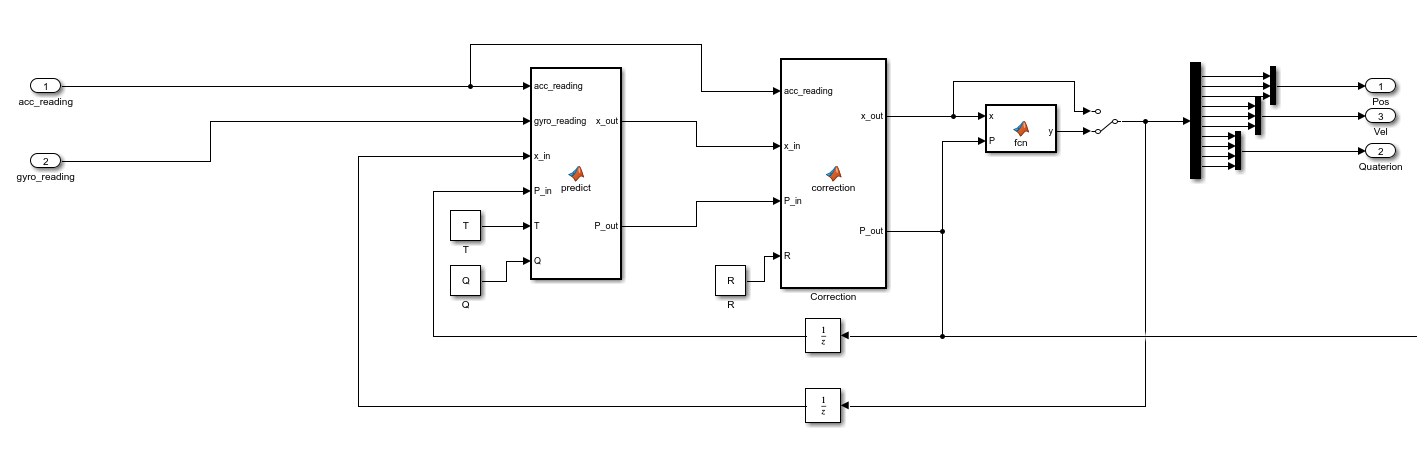
\includegraphics[width=0.9\textwidth]{duw/ekf.png}
	\caption{The Kalman Filter with constraints correction}
	\label{ekf_sim}
\end{figure}
\ \\

Thus prepared simulation was run multiple time to select an optimal set of parameters. The presented results are the best achieved after tuning process. First the filter work was examinated without the constraints' correction. A figure (\ref{no_con}) presents the coordinates change in function of time. The plot includes the robot's tip position, the moving platform's center's position and its estimation. The estimation (magenta, yellow and blue colors on plot) drifts heavily over simulation's time.\\

\begin{figure}[!h]
	\centering
	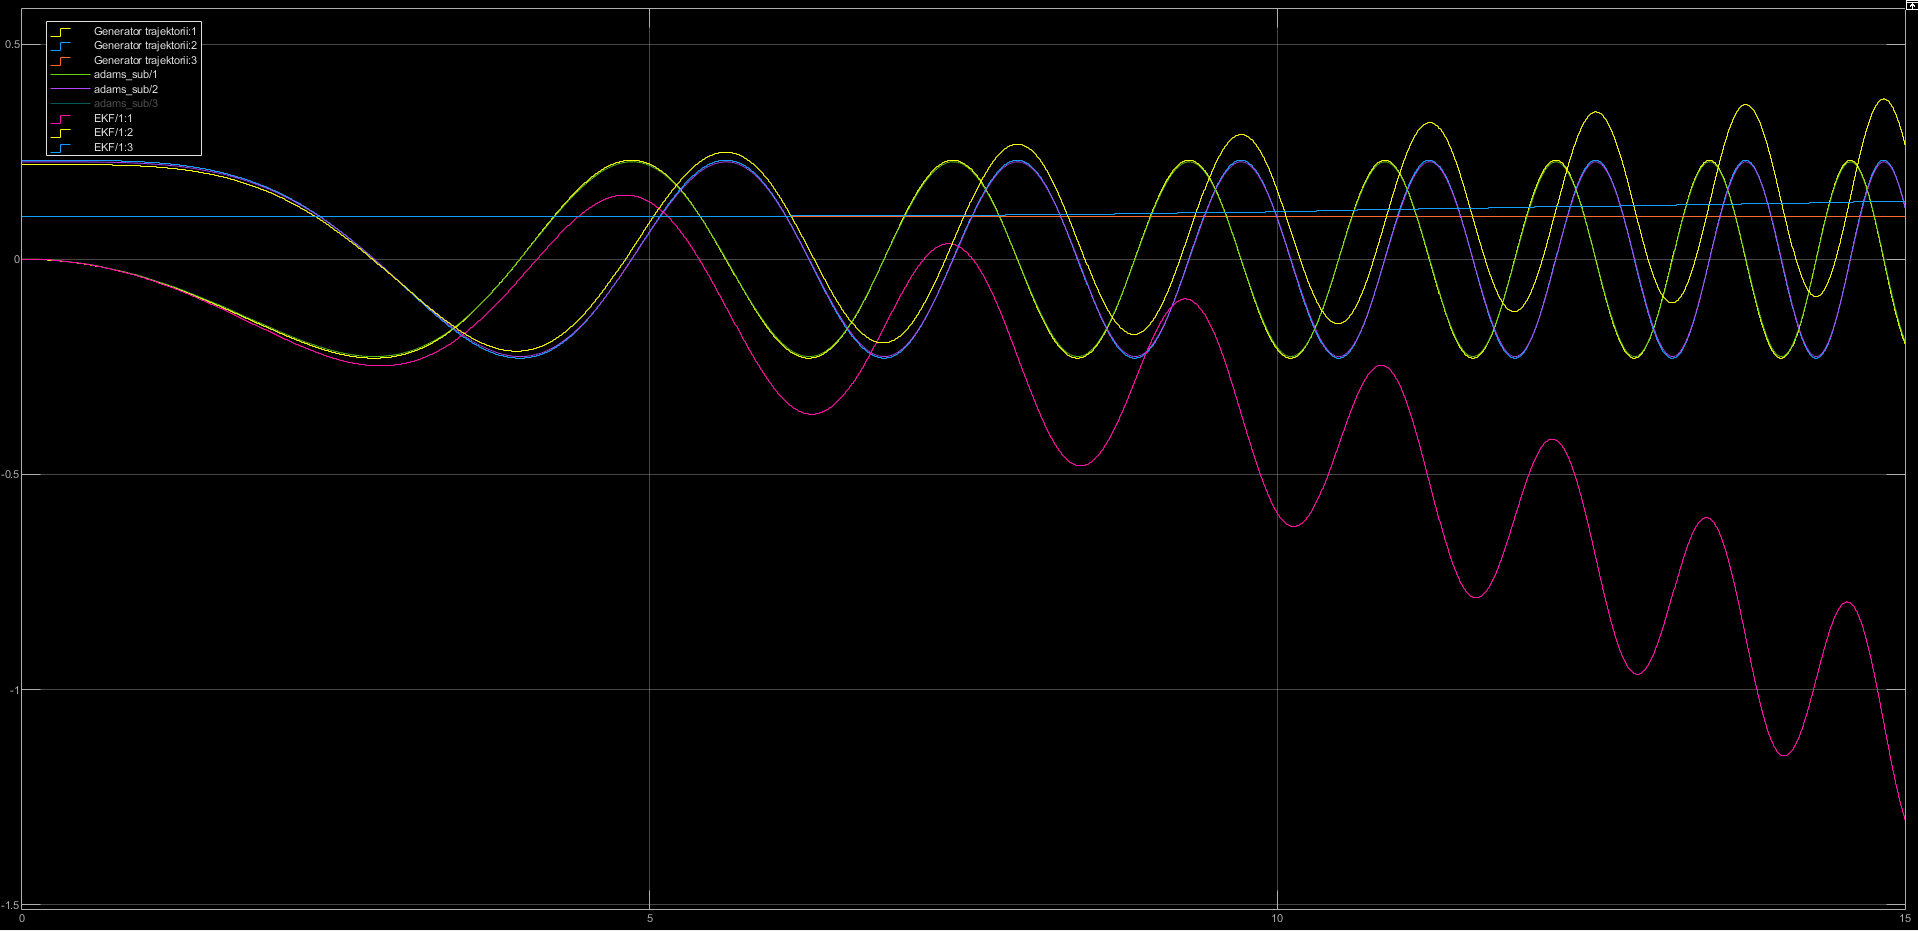
\includegraphics[width=\textwidth]{duw/no_con.png}
	\caption{The result of simulation (without correction)}
	\label{no_con}
\end{figure}

A figure (\ref{corr}) presents the run of same simulation, but with constraints' correction turned on. 
The estimation match the position for most of the simulation. During the second revolution the system lost tracked value but the match was quickly restored.

\begin{figure}[!h]
	\centering
	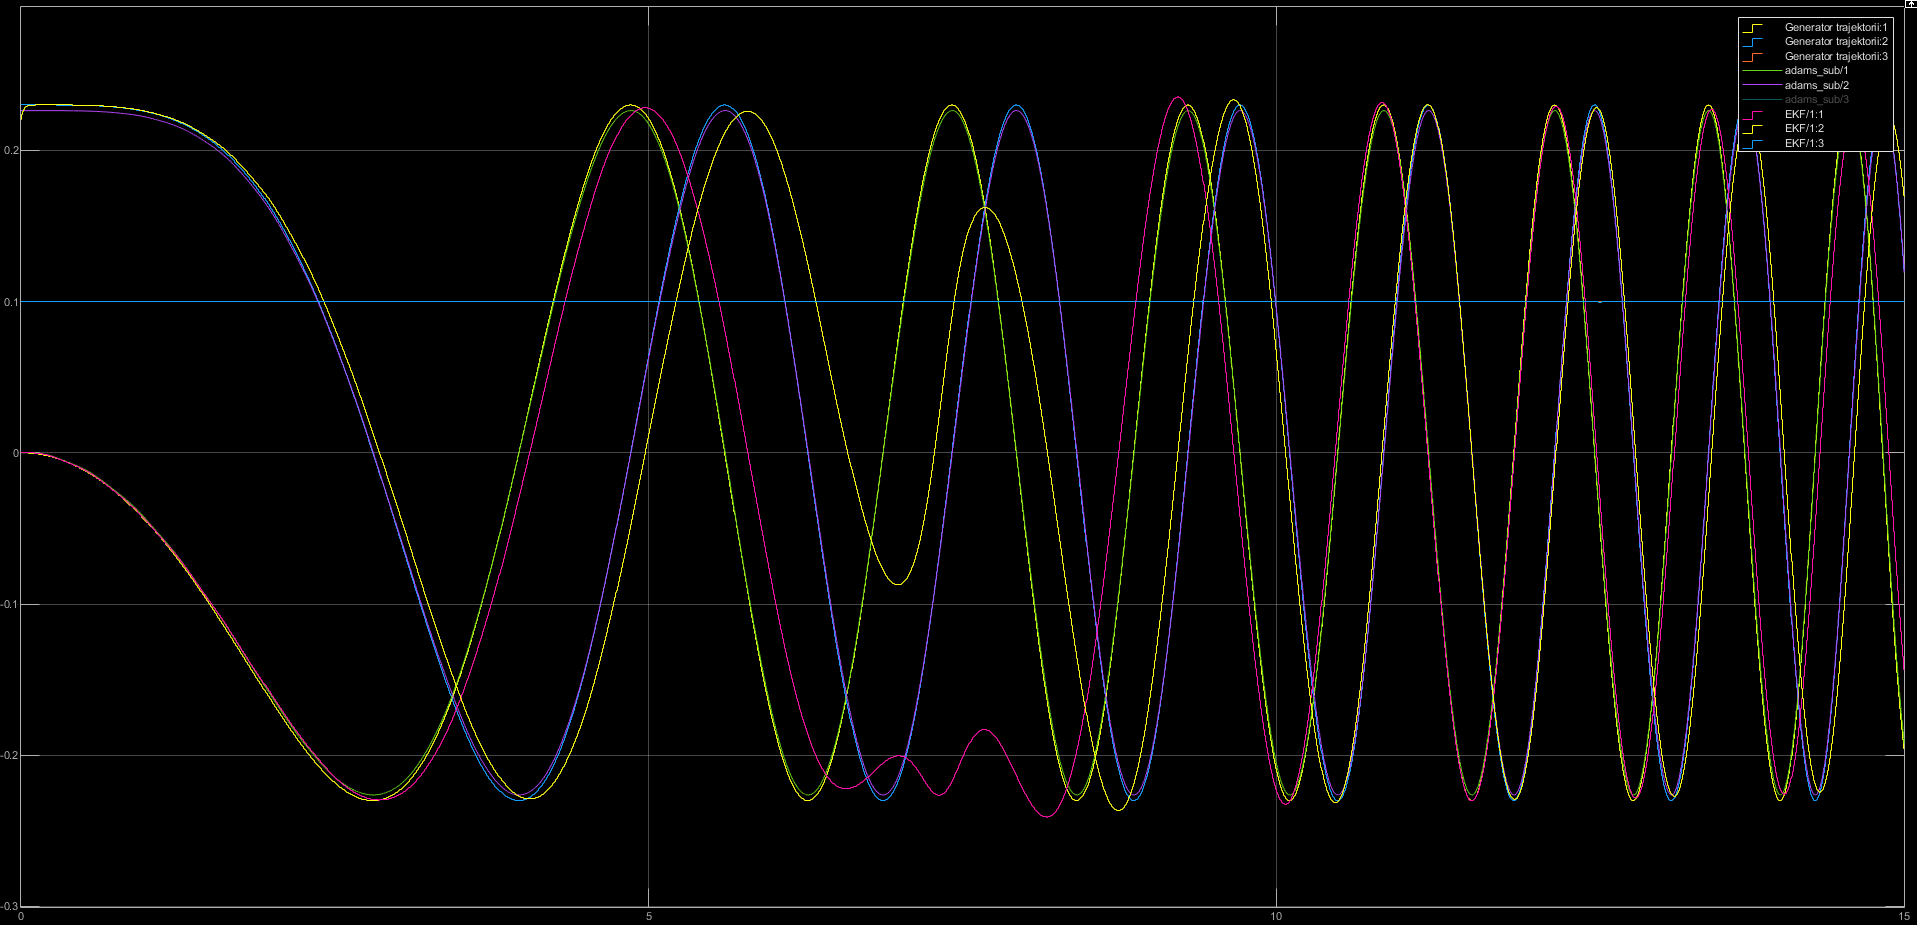
\includegraphics[width=\textwidth]{duw/corr.png}
	\caption{The result of simulation (with correction)}
	\label{corr}
\end{figure}

\newpage
Summarize, the simulation shows how positive is the impact of using the constraints' correction. Chronologically, the computer simulation was part of preparations for the realization of this thesis that energized the further work and complete system's implementation.

\chapter{Experiments}

\todo[inline, color=green]{
	Experiments: circular motion with different velocity in two direction, as in case study
}

\section{Results}

\todo[inline, color=green]{
	Comparation between:
	Position only, IMU only, IMU + constrainted, Position + constraints, Full working solution.
}

\chapter{Conclusion}

This thesis represents a comprehensive exploration of position and orientation estimation methods. Within the scope of this work, it was possible to gather extensive information about sensor fusion, data filtration, and signal processing. The thesis introduces a novel approach to utilize a knowledge of the system structure.\\

The developed system is a device that employs various sensors and seamlessly cooperates with application software. The system will be used for further research. For this reason, its operation has been further checked, and its correctness has been validated.\\

The present work opens the topic of using solutions taken from aviation and other technical sciences in the field of robot positioning. In particular, it is important to highlight the pioneering use of constraints correction in this field of science.


% This thesis enhances robotic positioning systems by integrating inertial navigation systems, inspired by aviation principles, with knowledge of mechanical design. The work done is part of a project being carried out at the Division of Theory of Machines and Robots. The primary goal is to fill a crucial gap in the existing setup – the absence of position and orientation sensors.\\

% The thesis explores fundamental navigation sensors, recognizing their limitations. It discusses strategies like filtering and sensor fusion to mitigate errors and obtain accurate position and orientation estimates. The proposed solution involves designing the experimental platform. This system modifies inertial navigation to estimate coordinates efficiently as the platform moves, addressing specific motion constraints.\\

% Anticipated outcomes include a deep understanding of position and orientation measurement systems and the design of a prototype tailored for robotic applications. This thesis may improve positioning systems, benefiting both the division's projects and the broader field of robotics.

\chapter{Bibliography}

%\printbibliography
%\nocite{*}

\printbibliography[type=article,heading=subbibliography,title={Articles}]
\printbibliography[type=online,heading=subbibliography,title={Online}]

% ----------------------- LIST OF SYMBOLS AND ABBREVIATIONS ------------------
\chapter*{List of symbols and abbreviations}

\todo[inline, color=green]{Fill in at the end}

\begin{tabular}{cl}
	nzw. & nadzwyczajny \\
	* & star operator \\
	$\widetilde{}$ & tilde 
\end{tabular}
\\
If you don't need it, delete it.
\thispagestyle{empty}

% -----------------------------  LIST OF APPENDICES ---------------------------
\chapter*{List of appendices}

\todo[inline, color=green]{Fill in at the end}

\begin{enumerate}
	\item MATLAB Scripts
	\item Appendix 2
	\item In case of no appendices, delete this part.
\end{enumerate}
\thispagestyle{empty}

\chapter*{Acknowledgment}

\todo[inline, color=green]{NCN OPUS 2023}


\end{document}